\documentclass[12pt,paper=a4]{report}
\usepackage[utf8]{inputenc}
\usepackage{polyglossia}
%Atkāpes pirmajām rindiņām
\usepackage{indentfirst}
%Virsrakstu noformējumam
\usepackage{titlesec}
%Attēlu importēšanai
\usepackage{graphicx}
%Vajadzēs saliktus attēlus
\usepackage{subcaption}
\usepackage{float}
%Nodefinē attālumus no malām
\usepackage[a4paper, lmargin=3.5cm,rmargin=2cm,tmargin=2cm, bmargin=2cm]{geometry}
%rotēšana
\usepackage{rotating, graphicx}
%Apjomīgām tabulām
\usepackage{longtable}
% tabulu šūnu satura centrēšanai
\usepackage{array}
\newcolumntype{P}[1]{>{\centering\arraybackslash}p{#1}}
\newcolumntype{M}[1]{>{\centering\arraybackslash}m{#1}}
%Numerācijai lappuses labajā pusē
\usepackage{fancyhdr}
%Literatūras saraksta veidošanai
%\usepackage{natbib}
\usepackage{hyperref} % For clickable links
\usepackage{url}      % For better URL formatting
\bibliographystyle{IEEEtran}

%Garas formulas
\usepackage{amsmath}

%tabulas
\usepackage{booktabs}
\usepackage{adjustbox}

% rindu sapludināšana tabulā
\usepackage{multirow}% http://ctan.org/pkg/multirow
\usepackage{hhline}% http://ctan.org/pkg/hhline
%laas tabulas
\usepackage{tabularx}
\usepackage{boldline}
%Lai varetu ievietot lapu landscape
\usepackage{lscape}
% pielikumam
\usepackage[titletoc]{appendix}
% Allows line breaks within cells
\usepackage{array}     % For column alignment
\usepackage{makecell}  % For line breaks in headers

\usepackage{pgfplots} % Required for plotting
\pgfplotsset{compat=1.18} % Ensure compatibility
\usepackage{siunitx} % For SI unit formatting

\usepackage{svg}
%Noformējuma parametri---------------------------------------------------------------------------------------------
%Nodefinējam valodas
\usepackage[labelsep=space]{caption} % Global setting for all tables
\setdefaultlanguage{latvian}
\setotherlanguages{english,russian}

%Fonts un atstarpe starp rindām
\setmainfont{Times New Roman}
%Rindiņas pirmā atkāpe
\setlength{\parindent}{1.27cm}
\usepackage{setspace}
\onehalfspacing
%Apakšmape bildēm
\graphicspath{{./pictures/}{./Schematics/}}

\renewcommand{\sfdefault}{ptm}

\titleformat{\chapter}
  {\centering\sffamily\fontsize{16}{16}\bfseries}{\thechapter \space{}}{0pc}{}
\titleformat{\section}{\sffamily\fontsize{14}{14}\bfseries}{\thesection \space{}}{0pc}{}
\titleformat{\subsection}{\sffamily\fontsize{12}{12}\bfseries}{\thesubsection \space{}}{0pc}{}
\titlespacing*{\chapter}{0pt}{0pt}{15pt} 
\titlespacing*{\section}{0pt}{20pt}{10pt} 
\titlespacing*{\subsection}{0pt}{15pt}{10pt} 

%Nodefinējam objektu numerācijas noteikumus
\def\thechapter      {\arabic{chapter}}
\def\thesection      {\ifx\chapter.\undefined{\arabic{section}}\else  {\thechapter.\arabic{section}}\fi}
\def\thesubsection   {\thesection.\arabic{subsection}}
\def\thesubsubsection{\thesubsection.\arabic{subsubsection}}

\usepackage{pdfpages}

\renewcommand{\thefigure}{\arabic{chapter}.\arabic{figure}.}
\renewcommand{\theequation}{\thechapter.\arabic{equation}.}
\renewcommand{\thetable}{\thechapter.\arabic{table}.}
%Attelu un tabulu nosaukumi
%\captionsetup[figure] {labelformat=default,labelsep=space,justification=centerlast}
%\captionsetup[table] {labelformat=simple,labelsep=newline,textfont=bf}
%\renewcommand{\figurename}{att.}

%\renewcommand{\tablename}{tabula}
%\renewcommand{\appendixname}{Pielikums}
%\makeatletter
%\renewcommand{\fnum@figure}{}
%\makeatother
%Teksta nodaļu fiksētie nosaukumi
\addto\captionslatvian{
\renewcommand\bibname{Izmantotās literatūras un avotu saraksts}
\renewcommand{\contentsname}{Saturs}
}

%Numeracija

\pagestyle{fancy}

\fancyhf{}
\renewcommand{\headrulewidth}{0pt} 
\renewcommand{\footrulewidth}{0pt}
\fancyfoot[R]{\thepage}
\fancypagestyle{plain}{%
  \fancyfoot[R]{\thepage}%
}
%Pārnesumiem - ļauj tiasīt lielākas starpas
\hyphenpenalty=5000
%% Atraitņrindiņas un bāreņrindiņas ( widow orphan) vadība
\clubpenalty10000
\widowpenalty10000
% Apakšsvītrām
\usepackage{underscore}
% pārkares paragrāfiem (speciāli saīsinājumiem)
\newenvironment{hangingpar}[1]
  {\begin{list}
          {}
          {\setlength{\itemindent}{-#1}%%'
           \setlength{\leftmargin}{#1}%%'
           \setlength{\itemsep}{0pt}%%'
           \setlength{\parsep}{\parskip}%%'
           \setlength{\topsep}{\parskip}%%'
           }
    \setlength{\parindent}{-#1}%%
    \item[]
  }
  {\end{list}}

%\renewcommand{\baselinestretch}{1.5}
\fontsize{12pt}{1.2}
\linespread{1.25} %1.2 *1.25 = 1.5

\begin{document}

% % Titullapa
\begin{titlepage}
\begin{center}
\textbf{
VENTSPILS AUGSTSKOLA\\
INFORMĀCIJAS TEHNOLOĢIJU FAKULTĀTE}\\
\vspace{1.2cm}
\textbf{BAKALAURA DARBS}\\
\vspace{1.4cm}
{\LARGE \textbf{X joslas raidīšanas sistēmas vadības bloka prototipa izstrāde}}\\
\vspace{1cm}
\begin{tabular}{@{}r@{}l@{}}
\parbox[c]{0.4\textwidth}{Autors:}&
\parbox[t]{0.6\textwidth}{
Ventspils Augstskola\\
Informācijas tehnoloģiju fakultātes\\
profesionālās bakalaura studiju programmas \\ "Elektronikas inženierija"\\
4. kursa students\\
Rodrigo Laurinovičs \\
Matrikulas~Nr. 190050 \vspace{0.7em}\\
\mbox{}\hrulefill\vspace{-0.4em}\\
{\scriptsize(paraksts)}\vspace{1.2cm}} \\
\parbox[c]{0.4\textwidth}{Fakultātes dekāns:}&
\parbox[t]{0.6\textwidth}{
doc. Dr.sc.comp. Vairis Caune \vspace{.7em}\\
\mbox{}\hrulefill\vspace{-0.4em}\\
{\scriptsize(paraksts)}\vspace{1.2cm}} \\
%-------------------------------------------------------------------------
\parbox[c]{0.4\textwidth}{Zinātniskais vadītājs:}&
\parbox[t]{0.6\textwidth}{
Mg. Sc. Ing. Mārcis Bleideris \vspace{.7em}\\
\mbox{}\hrulefill\vspace{-0.4em}\\
{\scriptsize(paraksts)}\vspace{1.2cm}} \\
%----------------------------------------------------------------------------------
\parbox[c]{0.4\textwidth}{Recenzents:} & %\vspace{.7em}\\
\parbox[t]{0.6\textwidth}{
Mg. Sc. Ing. Artūrs Orbidāns  \vspace{.7em}\\
%\mbox{}\hrulefill\vspace{-0.4em}\\

%{\scriptsize(Ieņemamais amats, zinātniskais nosaukums,
%vārds, uzvārds)}\vspace{2em}

\mbox{}\hrulefill\vspace{-0.4em}\\
{\scriptsize(paraksts)}\vspace{2em}} \\
\end{tabular}
\vfill
Ventspils, 2025
\end{center}
\end{titlepage}
\pagenumbering{gobble}
%Vieta anotācijām---------------------------------------------------------------------------
\chapter*{ANOTĀCIJA}
\begin{flushleft}
\textbf{Darba nosaukums:} X joslas raidīšanas sistēmas vadības bloka prototipa izstrāde.\\
\textbf{Darba autors:} Rodrigo Laurinovičs\\
\textbf{Darba vadītājs:} Mg. Sc. Ing. Mārcis Bleiders\\
\textbf{Darba apjoms:} 38.lpp, 5 tabulas, 51 attēli, 31 bibliogrāfiskās norādes, 0 pielikumi\\
\textbf{Atslēgas vārdi:} X-joslas raidītāja darba punkta iestatīšana, RMS jaudas detektors, TCP/IP, satelīta komunikācija\\

Bakalaura darbā izstrādāts funkcionējošs darba punkta un lieljaudas pastiprinātāja monitorēšanas prototips, kas ir vadāms caur tīklu un pielietojams raidītāja vadīšanai satelīta komunikācijās X diapazonā.\\

Darbā aprakstītas RT-16 X diapazona sistēma, dziļā kosmosa komunikāciju sadalījums, jaudas pastiprinātāju esošās vadības sistēmas, jaudas detektori. Definēti sasniedzamie parametri un funkcionalitāte, kas jāpielāgo raidītāju efektīvai izmantošanai Irbenes esošajā radioteleskopu sistēmā.\\

Prototipēšanas atvieglošanas nolūkos katra apakšsistēma izstrādāta kā neatkarīgs modulis, izmantojot mūsdienīgas, viegli pieejamas elektronikas komponentes un materiālus. Izstrādātās moduļu principiālās shēmas izstrādē tika izmantoti datorizēti izstrādes rīki. Izgatavotām apakšsistēmām veikti to raksturīgāko elektrisko parametru mērījumi.\\

Izveidotais prototips notestēts raidīšanas sistēmā, veikti tās veiktspēju raksturojošo parametru mērījumi, pārbaudīta sasniegtā funkcionalitāte un izdarīti secinājumi.
\end{flushleft}


\chapter*{ABSTRACT}
\begin{flushleft}
\textbf{Title:} Prototype development of the control unit for the X band transmission system\\
\textbf{Author:} Rodrigo Laurinovičs\\
\textbf{Supervising tutor:} Mg. Sc. Ing. Mārcis Bleiders\\
\textbf{Scope of work:} 38 pages, 5 tables, 51 figures, 32 bibliographical references, 0 appendices.
\textbf{Keywords:} X-band transmitter bias-up and bias-down, True RMS power detectors, TCP/IP, satellite communications
\\In the bachelor's thesis, a functional prototype for monitoring and biasing a high-power amplifier has been developed. The prototype is network-controllable and applicable for transmitter control in satellite communications in the X-band.\\

The paper describes the RT16 X-band system, the spectrum allocation of the Deep Space Network, existing control systems for power amplifiers, and power detectors. The achievable parameters and functionality required for the efficient use of transmitters in the existing Irbene radio telescope system have been defined.\\

To facilitate prototyping, each subsystem was developed as an independent module using modern, easily accessible electronic components and materials. Computer-aided design tools were used in the development of the module schematics.\\

Measurements of the key electrical parameters were performed on the manufactured subsystems. The prototype was tested in a transmission system, with performance-related parameter measurements conducted, achieved functionality verified, and conclusions drawn.
\end{flushleft}

%Saturs---------------------------------------------------------------------------------------
\tableofcontents
\newcommand{\abbreviation}[3]{%
    \makebox[4em][l]{#1} --  #2 (\textit{#3})\par
}

\chapter*{Saīsinājumi un to klasifikācija}
\begin{hangingpar}{4em}
\abbreviation{ESA}{Eiropas Kosmosa aģentūra}{European Space Agency}
\abbreviation{SPI}{Seriālā perifērā saskarne}{Serial Peripheral Interface}
\abbreviation{VSRC}{Ventspils Starptautiskais Radioastronomijas Centrs}{Ventspils International Radio Astronomy Centre}
\abbreviation{RF}{Radiofrekvence}{Radio frequency}
\abbreviation{GaN}{Gallija nitrīds}{Gallium Nitride}

\end{hangingpar}
\clearpage
\pagenumbering{arabic}
\setcounter{page}{6}
\chapter{Ievads}
Ventspils Starptautiskā Radioastronomijas Centra (\textit{VSRC}) rīcībā ir teleskopi RT-16 un RT-32, kas vēsturiski tika izmantoti rietumu pasaules spiegošanā, bet pašlaik ir zinātnes instruments kosmosa izpētē. VSRC zinātniskajā institūtā pašlaik notiek darbs pie radioteleskopu komercializācijas, izmantojot antenas kā bāzes stacijas satelītu un kosmosa izpētes misijām, t.sk uz Mēness. Šim nolūkam tiek veidots S/X diapazona raiduztvērējs RT-16 radioteleskopam, kur daļa no tā ir X diapazona (No 7.25 GHz līdz 7.75 GHz) raidītājs, ko izstrādā darba vadītājs Mārcis Bleideris. Raidītāja vadībai ir jaizstrādā vadības bloka risinājums, kas ietver sistēmas ieslēgšanu, izslēgšanu X joslas 100 W Gallija nitrīda (\textit{GaN}) jaudas pastiprinātāja (\textit{HPA}) modelim (QPM1017) un elektrobarošanas avotiem. Vadības bloks ir nepieciešams, lai pasargātu augstas jaudas pastiprinātāju no pārkaršanas, pārsprieguma, pārstrāvas vai nesaskaņotas slodzes pretestības radītiem riskiem, kas var radīt neatgriezeniskus iekārtas bojājumus. 
Bakalaura darba mērķa sasniegšanai, tika izvirzīti šādi uzdevumi:
\begin{itemize}
    \item Izpētīt esošās jaudas pastiprinātāju vadības sistēmas;
    \item Piemeklēt specifikācijai piemērotu risinājumu;
    \item Izveidot testa stendu;
    \item Izstrādāt funkcionējošu maketu, kuru var vadīt caur ethernet tīklu;
    \item Izstrādāt iespiedpalti, piemērotu VSRC vajadzībām;
    \item Saintegrēt to eksistējošā korpusā.
\end{itemize}
Turpmāk darbs tiek sadalīts vairākās daļas: teorijā, izstrādē un testēšanā. Teorijā tiek padziļinātāk apskatīts idejas koncepts, apskatīties risinājumi un izvēlētā risinājuma teorētiskais pamatojums. Izstrādē tiek detalizēti izsklāstīts iekārtas veidošanas process no izstrādes platei līdz paštaisītam risinājumam ar nepieciešamajām funkcionalitātēm. Testēšanā tiek pārbaudīta iekārtas atbilstība norādītajai specifikācijai.


\chapter{Teorija}

Šajā nodaļā tiek apskatīti jaudas pastiprinātāji, to vadības sistēmas, izstarotās un atstarotās jaudas detektori, kā arī piedāvātie risinājumi vadības sistēmām, jaudas detektoriem un izvēlētie risinājumi pastiprinātājam, vadības sistēmai un jaudas noteikšanai.

\section{"Koncepts"}
\subsection{Augstas jaudas RF pastiprinātāji}
Augstas jaudas RF pastiprinātāji ir būtisks sastāvdaļā bezvadu sistēmās. To uzdevums ir pastiprināt signālus jaudu, ļaujot tos pārraidīt lielākos attālumos. Šie pastiprinātāji tiek izmantoti dažādās nozarēs, tostarp satelītu sakaros.

Tipisks augstas jaudas RF pastiprinātājs sastāv no vairākām daļām, kuras veic dažādas signāla pastiprināšanas un kondicionēšanas funkcijas. 

Galvenās sastāvdaļas ir:
\begin{itemize}
    \item Ieejas tīkla saskaņošana;
    \begin{itemize}
        \item Nodrošina maksimālu enerģijas pārnesi no signāla avota uz pastiprinātāju;
        \item Pielāgo ieejas signāla avota pretestību pastiprinātāja pirmajai pakāpei;
    \end{itemize}
    \item Priekšpastiprinātājs;
    \begin{itemize}
        \item Nodrošina sākotnējo signāla pastiprināšanu ar nelielu pastiprinājumu;
        \item Maztrokšnojoša pakāpe;
    \end{itemize}
    \item Vidējās jaudas pastiprinātājs;
    \begin{itemize}
        \item Veic lielāko daļu signāla pastiprināšanas;
        \item Parasti sastāv no vairākām tranzistoru pakāpēm kaskādes vai paralēlā konfigurācijā;
        \item Var ietvert atgriezeniskās saites shēmas linearitātes un stabilitātes uzlabošanai; 
    \end{itemize}
    \item Gala jaudas pastiprinātājs (izejas pakāpe):
    \begin{itemize}
        \item Nodrošina visaugstāko jaudas līmeni, bieži diapazonā no W līdz kW.;
        \item Izmanto augstas jaudas tranzistorus (piem., MOSFET, GaN HEMT vai LDMOS) vai vakuuma lampas;
        \item Jānodrošina efektīvu siltuma izkliedi, jo rada lielu enerģijas zudumu siltumā.
    \end{itemize}
    \item Izejas saskaņošanas tīkls:
    \begin{itemize}
        \item Saskaņo pastiprinātāja izejas pretestību ar slodzi (piem., antenu vai pārraides līniju);
        \item Nodrošina efektīvu jaudas pārnesi un samazina signāla atstarojumus.
    \end{itemize}
    \item Barošanas avoti un darba punkta iestatīšanas shēmas:
    \begin{itemize}
        \item Nodrošina nepieciešamo līdzstrāvas barošanu aktīvajām komponentēm;
        \item Var ietvert sprieguma stabilizatorus, DC-DC pārveidotājus un darba punkta iestatīšanas tranzistoriem.
    \end{itemize}
     \item Dzesēšanas sistēma:
     \begin{itemize}
        \item Izmanto radiatorus, ventilatorus vai šķidruma dzesēšanas sistēmas termiskās stabilitātes nodrošināšanai.
    \end{itemize}
\end{itemize}

Augstas jaudas RF pastiprinātājus var klasificēt pēc to darbības režīma un efektivitātes:
\begin{itemize}
    \item A klase: Augsta linearitāte, bet zema efektivitāte (~25-30\%). Izmanto pielietojumos, kur nepieciešama minimāla signāla kropļošana;
    \item B/AB klase: Uzlabota efektivitāte (~50-70\%) ar nelielu nelinearitāti, bieži lieto apraides raidītājos;
    \item C klase: Augsta efektivitāte (~75-85\%), piemērota pielietojumiem, kur neliela signāla kropļošana nav kritiska, piemēram, FM raidītājos;
    \item D/E/F klase: pastiprinātāji ar efektivitāti virs 90\%, izmanto specializētās RF pielietojumos.
\end{itemize}

% atsauces:
% Pozar, D. M. (2011). Microwave Engineering (4th ed.). Wiley.
% Krauss, H. L., Bostian, C. W., & Raab, F. H. (1980). Solid State Radio Engineering. Wiley.
% Cripps, S. C. (2006). RF Power Amplifiers for Wireless Communications (2nd ed.). Artech House.

\subsection{Vadības sistēmas RF jaudas pastiprinātājiem}
Lai gan RF jaudas pastiprinātāji ir atbildīgi par signāla pastiprināšanu, vadības sistēma ir tā, kas nodrošina to optimālu darbību, precīzu jaudas regulēšanu un aizsardzību pret iespējamiem darbības traucējumiem.
RF jaudas pastiprinātājiem ir nepieciešama vadības sistēma vairāku iemeslu dēļ:
\begin{itemize}
    \item Jaudas regulēšana: RF pastiprinātājiem jāspēj dinamiski pielāgot savu jaudu atkarībā no ārējiem faktoriem, piemēram, signāla kvalitātes, tālāka pārraides attāluma vai apkārtējās vides apstākļiem;
    \item Aizsardzība pret pārslodzi: RF pastiprinātāji var tikt bojāti pārmērīgas jaudas dēļ. Vadības sistēma var uzraudzīt pastiprinātāja darbību un aktivizēt aizsardzības režīmus, piemēram, automātisku izslēgšanu vai jaudas samazināšanu, lai novērstu bojājumus;
    \item Efektivitāte un enerģijas patēriņš: Ar efektīvu vadības sistēmu iespējams uzlabot pastiprinātāja energoefektivitāti, optimizējot darbības apstākļus, samazinot liekās enerģijas patēriņu un palielinot sistēmas darbības ilgumu;
\end{itemize}

RF jaudas pastiprinātāju vadības sistēmas tiek pielietotas vairākās jomās:

\begin{itemize}
    \item Telekomunikācijas - Vadības sistēma palīdz pielāgot jaudu atbilstoši tīkla apstākļiem, lai nodrošinātu optimālu pārraidi un izvairītos no traucējumiem;
    \item Kosmosa un satelītu tehnoloģijas - Vadības sistēma ļauj uzraudzīt jaudas līmeni un pielāgot to, ņemot vērā vides apstākļus, piemēram, atmosfēras traucējumus;
    \item Radar sistēmas - Vadības sistēma nodrošina, ka radarā tiek izmantota optimāla jauda, lai uzlabotu precizitāti un samazinātu traucējumus;
    \item RFID un bezvadu sensoru tīkli - Vadības sistēma palīdz regulēt jaudu un nodrošina efektīvu enerģijas patēriņu.;
\end{itemize}

Vadības sistēmas RF jaudas pastiprinātājiem tiek implementētas vairākos veidos:
\begin{itemize}
    \item Automātiskā jaudas regulēšana (AGC) - AGC ir bieži izmantota tehnoloģija, kas ļauj automātiski pielāgot pastiprinātāja jaudu, lai uzturētu optimālu signāla līmeni;
    \item Digitālie signālu procesori (DSP) - Vadības sistēmas bieži izmanto DSP tehnoloģijas, lai apstrādātu un analizētu RF signālus reālajā laikā. DSP ļauj veikt precīzu signāla analīzi un uzraudzību, kas nepieciešama, lai regulētu jaudu un nodrošinātu augstu pārraides kvalitāti;
    \item Vairāku sensoru izmantošana - Lai uzraudzītu dažādus parametrus, piemēram, temperatūru, spriegumu un strāvu, tiek izmantoti vairāki sensori, kas darbojas kopā ar vadības sistēmu, lai nodrošinātu pastiprinātāja aizsardzību un efektīvu darbību;
    \item Kompleksi algoritmi un kontrolējošas loģikas sistēmas - Vadības sistēmas var ietvert algoritmus, kas ņem vērā daudzus faktorus, piemēram, apkārtējo traucējumu līmeni, sistēmas pieprasījumu un jaudas pieejamību. Šie algoritmi ļauj pielāgot pastiprinātāja darbību un uzlabot sistēmas veiktspēju;
\end{itemize}

RF jaudas pastiprinātāji ir svarīgi sastāvdaļa modernās komunikāciju sistēmās, un to efektīva darbība ir atkarīga no labi izstrādātām vadības sistēmām. Šādas sistēmas nodrošina jaudas regulēšanu, aizsardzību, enerģijas efektivitāti un augstu signāla kvalitāti, kas ir nepieciešama daudzās nozarēs, sākot no telekomunikācijām līdz kosmosa tehnoloģijām. Ar vienkāršotu.

\subsection{Teorētiska un tehniskā skaidrojums par izstaroto un atstarotā jaudas detektoriem (Prefl un Pfwd detektoriem)}
P\textsubscript{refl} un P\textsubscript{fwd} noteikšanas shēmas tiek izmantotas RF sistēmās, lai uzraudzītu izstaroto un atstaroto jaudu pārvades līnijā. Šie mērījumi ir būtiski, lai nodrošinātu, ka sistēma darbojas efektīvi. P\textsubscript{refl} attiecas uz atstaroto jaudu uz jaudas pastiprinātāju un P\textsubscript{fwd} attiecas uz izstaroto jaudu no jaudas pastiprinātāja.

\subsubsection{Atstarotās P\textsubscript{refl} jaudas detektori}
Atstarotā jauda ir signāla daļa, kas tiek atgriezta avotā pretestības neatbilstību vai atstarojumu dēļ pārraides līnijā. Atstarotās jaudas noteikšana ir svarīga, lai nodrošinātu, ka sistēma nepiedzīvo ievērojamus zaudējumus atstarošanas dēļ, kas var sabojāt komponentes vai izraisīt neefektivitāti.

Atstarotās jaudas detektora tipi:
\begin{itemize}
    \item \textbf{Uz virziena savienotāju balstīta noteikšana (Directional Coupler-based Detection)};
\end{itemize}

Virziena savienotājs ir visizplatītākā metode atstarotās jaudas mērīšanai. Tas ņem paraugus no nelielas atstarotā signāla daļas un novirza to uz detektoru, parasti diodi vai RF barošanas sensoru.

Virziena savienotājs sadala tajā ienākošo jaudu divos ceļos. Signāls, kas pārvietojas virzienā uz priekšu, tiek savienots no viena porta (izstarotā jauda), bet atstarotais signāls tiek savienots no cita porta (atstarotā jauda). Šo jaudu attiecību nosaka savienotāja konstrukcija, un atstarotā jauda tiek noteikta caur saistītu portu, kas atbilst atstarojumam.
Priekšrocības:
\begin{itemize}
    \item Precīzs un vienkāršs;
    \item Nodrošina vienlaicīgus izstarotā un atstarotā jaudas mērījumus;
    \item Bieži un plaši izmanto sakaru sistēmās.
\end{itemize}
Mīnusi:
\begin{itemize}
    \item Frekvences reakcija ir atkarīga no savienotāja konstrukcijas;
    \item Savienotāja zudums (insertion loss) var samazināt mērījumu precizitāti.
\end{itemize}

\begin{itemize}
    \item \textbf{(Bridge-based Detection [Wheatstone Bridge or Impedance Bridge])};
\end{itemize}
Šī metode izmanto tilta slēgumu, lai izmērītu atstaroto jaudu. Šādās ķēdēs atstarošana izraisa sprieguma nelīdzsvarotību, ko var noteikt, bieži vien izmantojot diodi vai citu taisngriešanas elementu.

Līdzsvarota tilta slēgumā izmanto pretestības saskaņošanas principu, lai noteiktu atstarojumus. Ja nav atspulga (perfekta atbilstība), tilts ir līdzsvarots, un signāla atšķirība neveidojas. Kad rodas atstarojumi, pretestības neatbilstība izraisa nelīdzsvarotību.

Priekšrocības:
\begin{itemize}
    \item Augsta jutība pret nelielām atstarotās jaudas variācijām;
    \item Var strādāt plašā frekvenču diapazonā.
\end{itemize}
Mīnusi:
\begin{itemize}
    \item Augstāka sarežgītība salīdzinot ar citām metodēm;
    \item Jutīgi pret dreifēšanu, īpaši ar temperatūras izmaiņām.
\end{itemize}

\begin{itemize}
    \item \textbf{Diožu jaudas detektori (Diode-based Detectors)}.
\end{itemize}
Vienkāršu diodes detektoru var izmantot kopā ar virziena savienotāju vai tiltu, lai tieši izmērītu atstaroto jaudu.

Diodes taisngriezis uztver RF signālu un pārvērš to līdzstrāvas signālā, ko var izmērīt ar atbilstošu skaitītāju. Līdstrāvas spriegums ir proporcionāls atstarotā signāla jaudas līmenim.

Priekšrocības:
\begin{itemize}
    \item Vienkāršā un rentabla (cost-effective);
    \item Nodrošina atstarotās jaudas mērīšanu reālā laikā.
\end{itemize}
Mīnusi:
\begin{itemize}
    \item Precizitāti ierobežo diodes nelinearitāte, īpaši lieljaudas signāliem;
\end{itemize}

\subsubsection{Izstarotās P\textsubscript{fwd} jaudas detektori}
Izstarotā jauda tiek piegādāta no avota uz antenu vai citu patērētāju. Ir nepieciešams monitorēt izstaroto jaudu, lai novērtētu jaudas pastiprinātāja pastiprinājuma koeficientu un vai darbība ir optimāla.

\begin{itemize}
    \item \textbf{Termiskās jaudas noteicējs (Thermal Power Detectors)};
\end{itemize}
Šie detektori mēra signāla radīto siltumu, kad tas iet caur pretestību. Sildīšanas efekts ir proporcionāls piegādātajai jaudai, un termistors vai termopāris var pārvērst šo temperatūras maiņu lasāmā signālā.

Termiskais detektors mēra temperatūras paaugstināšanos pretestībā, ko izraisa RF signāla izkliedētā jauda. Šī metode ir diezgan precīza, jo tā tieši mēra faktisko jaudu, taču tā relatīvi lēna, un tai nepieciešama rūpīga kalibrēšana.

Priekšrocības:
\begin{itemize}
    \item Precīzs un nodrošina absolūtus jaudas mērījumus;
    \item Var izmērīt gan  izstaroto, gan atstaroto jaudu.
\end{itemize}
Mīnusi:
\begin{itemize}
    \item Lēns reakcijas laiks, kas neatļauj izmantot augstās frekvenču aplikācijās.;
\end{itemize}

\begin{itemize}
    \item \textbf{Diožu jaudas detektori (Diode-based Detectors)};
\end{itemize}
Līdzīgi kā atstarotās jaudas noteikšanā, arī izstaroto jaudu var noteikt, taisngriežot signālu, izmantojot diodes. Signāla ceļā tiek ievietots diodes detektors, un, tā kā diode taisno RF signālu, iegūtais līdzstrāvas spriegums ir proporcionāls momentānajai jaudai.

Priekšrocības:
\begin{itemize}
    \item Vienkārši un lēti;
    \item Ātrs reakcijas laiks.
\end{itemize}
Mīnusi:
\begin{itemize}
    \item Precizitāti var ierobežot diodes īpašības, īpaši augstfrekvences signāliem;
    \item Nepieciešama kalibrēšana dažādiem signālu tipiem.
\end{itemize}

\begin{itemize}
    \item \textbf{Pīķa detektori (Peak Detectors)}.
\end{itemize}
Pīķa detektorus var izmantot sistēmās, kurās jāuzrauga tikai maksimālā jauda. Šie detektori uztver maksimālo momentāno jaudu, bieži izmantojot diodes un kondensatora kombināciju, lai saglabātu maksimālo vērtību.

Maksimālais detektors uztver un notur ieejas signāla maksimālo vērtību. Kad signāls sasniedz maksimumu, kondensators uzlādējas līdz noteiktam spriegumam, un līdzstrāvas izeja atspoguļo maksimālo jaudas līmeni.

Priekšrocības:
\begin{itemize}
    \item Ātra reakcija un precīzi pīķa mērījumi;
    \item Noderīga signāliem ar pārejošiem impulsu RF signāliem.
\end{itemize}
Mīnusi:
\begin{itemize}
    \item Nenodrošina vidējo jaudas vērtību;
    \item Var būt mazāk efektīvs nepārtrauktiem signāliem bez būtiskiem pīķiem.
\end{itemize}

Kuras metodes izmanto kādiem pielietojumiem:
\begin{itemize}
    \item Komunikācijas sistēmās - Uz virziena savienotāju balstīta noteikšana (Directional Couplers);
    \item Augstas jaudas sistēmās (raidītājos, jaudas pastiprinātājos) - Termiskais detektors(Thermal Detectors);
    \item Signāla monitorēšanai un atkļūdošanai - Diožu detektors (Diode-base detector);
    \item Mērījumu iekārtām - Tilta detektori (Bridge-based detection circuits).
\end{itemize}

%atsauces
% Gupta, R. S., & Wadhwa, M. (2014). "Microwave Engineering." - This text provides detailed theoretical explanations and practical applications for various types of RF power detectors, including directional couplers and diode detectors.
% Pozar, D. M. (2012). "Microwave Engineering" (4th ed.). - Offers an in-depth explanation of impedance matching and directional coupler theory, relevant to reflected and forward power detection.
% Krauss, J. D. (2011). "RF and Microwave Radiation Safety." - Covers methods and challenges in power measurement, including forward and reflected power detection in RF systems.

\section{"Apskatītie risinājumi"}
\subsection{Vadības integrālās shēmas priekš jaudas pastiprinātāji}
\begin{table}[h]
    \centering
    \renewcommand{\arraystretch}{1.3}
    \setlength{\tabcolsep}{5pt} % Adjust column spacing
    \begin{adjustbox}{max width=\textwidth}
    \begin{tabular}{|p{3cm}|p{3cm}|p{3cm}|p{3cm}|p{4cm}|}
        \hline
        \textbf{Integrālā shēma} & \textbf{Funkcijas} & \textbf{Pielietojums} & \textbf{Spriegums} & \textbf{Atšķiras} \\
        \hline
        Analog Devices AD7293 & Darba punkta iestatīšana un aizsardzība & RF pastiprinātāju vadība, signālu uzraudzība un aizsardzība & 3.3V -- 5.5V & Integrēts ADC un DAC, termālā aizsardzība, sprieguma un strāvas uzraudzība, trauksmes izvadi \\
        \hline
        Texas Instruments ADC12D1800 & 12-Bitu, 1.8 GSPS Datu pārveidotājs & RF sistēmas ātrai signālu nolasei un uzraudzībai & 3.3V & Ātra nolase, zems enerģijas patēriņš un augsta nolases izšķirtspēja \\
        \hline
        Maxim MAX11200 & 24-Bitu, 4-kanālu ADC ar iebūvētu multiplikatoru & Signālu iegūšanai RF pastiprinātāju vadībā & 2.7V -- 5.5V & Augsta precizitāte, zema enerģija, integrēta multiplikatora funkcionalitāte \\
        \hline
        Analog Devices AD5700 & 16-Bitu, 4-kanālu signālu iegūšanas sistēma & RF sistēmu signālu mērīšanai un kontrolei & 3.0V -- 5.5V & Precīzi signālu mērījumi, integrēti trauksmes izvadi, termālā aizsardzība \\
        \hline
        Linear Technology LTC2378-16 & 16-Bitu, 8-kanālu ADC ar iebūvētu multiplikatoru & RF signālu mērīšanai un uzraudzībai & 2.7V -- 5.5V & Augsta precizitāte, zema trokšņa veiktspēja, integrēti trauksmes izvadi \\
        \hline
        Maxim MAX14733 & 16-Bitu, vairāku kanālu ADC ar iebūvētu multiplikatoru & RF signālu uzraudzībai un vadības sistēmām & 3.0V -- 5.5V & Vairāku kanālu signālu iegūšana, zems trokšņu līmenis, trauksmes izvadi \\
        \hline
        Texas Instruments ADS8900B & 16-Bitu, vienkanālu, zema enerģijas ADC & Precīzai signālu uzraudzībai RF pastiprinātāju vadībā & 2.7V -- 5.5V & Zems aizkaves laiks, programmējami trauksmes sliekšņi un reālā laika monitorēšanai \\
        \hline
        Analog Devices AD7779 & 24-Bitu, vairāku kanālu Sigma-Delta ADC ar trauksmes izvadiem & RF sistēmu signālu uzraudzībai un vadībai & 2.7V -- 5.5V & Augsta izšķirtspēja un precizitāte, vairāku kanālu atbalsts, integrēti trauksmes izvadi \\
        \hline
    \end{tabular}
    \end{adjustbox}
    \caption{GaN pastiprinātāju vadības bloku mikroshēmu piemēri un salīdzinājums}
    \label{tab:gan_control_blocks}
\end{table}

No apskatītajiem RF jaudas vadības integrālajām shēmām tika  izvēlēta Analog Devices ražojums "AD7293" salīdzinoši lētās izmaksas dēļ un nodrošina visu nepieciešamo funkcionalitāti pēc VSRC specifikācijām.

\subsection{Izstarotās un atstarotājs jaudas aktīvās RMS jaudas detektors (true RMS power detector)}
Virziena savienotāji izmanto, lai izmērītu gan izstaroto, gan atstaroto jaudu. Virziena savienotājs ir pasīva četru portu ierīce, kas ļauj enerģiju no vienas pārvades līnijas kontrolētā veidā pārnest uz otru pārvades līniju. Tas atdala signālu divās komponentēs: viens ir izstarotā jauda (plūst tajā pašā virzienā kā signāls), bet otrs ir atstarotā jauda (kas plūst atpakaļ uz avotu, ja ir pretestības neatbilstība).

Virziena savienotājs sastāv no četriem portiem:
\begin{itemize}
    \item Ieejas ports - Tas ir ports, kurā signāls tiek ievadīts savienotājā no raidītāja;
    \item Izejas ports - Ieejas signāla izeja, kas tiek nogādāta uz patērētāju, piemēram, antēnu.
    \item Saistīts port (coupled port) - Šī ir pieslēgvieta, kas ir proporcionāls ieejas jaudai. Tas mēra tiešo jaudu līnijā.
    \item Atsaistīts ports (isolated port) - Šis ports saņem atstaroto signālu, kas ir proporcionāla atstarotajam signālam.
\end{itemize}

Darbības princips:
\begin{itemize}
    \item Izejošās jaudas noteikšānai - Ievades signāls nonāk 1. portā, un lielākā daļa no tā iziet no 2. porta. Neliela signāla daļa tiek padota uz 3 portu.
    \item Atstarotās jaudas noteikšānai - Atstarotā jauda ceļo atpakaļ savienotāju, kur daļa no tā tiek padota 4 portā.
\end{itemize}

Virziena savienotāji balstās uz jaudas dalīšanas un savienošanas principu, izmantojot elektromagnētiskos laukus. Šie savienotāji ir paredzēti darbam plašā frekvenču diapazonā, un saites koeficients (coupling factor) nosaka jaudas daudzumu, kas tiek pārnests uz savienoto portu.

\begin{itemize}
    \item \textbf{saites koeficients}
\end{itemize}
Saites koeficients nosaka, cik liela daļa signāla ir "savienota" no galvenās pārraides līnijas uz savienoto līniju. To parasti izsaka dB (decibelos). Piemēram, 20 dB savienotājs nodod 1/100 daļu no ieejas jaudas uz savienoto portu.
Saites koeficientu definē šādi:
\[
C = 10log(\frac{Pinput}{Pcoupled})
\]
, kur
\begin{itemize}
    \item Pinput ir savienotāja ieejas jauda.
    \item Pcoupled ir jauda, kas savienota ar portu 3 (tiešajai jaudai) vai portu 4 (atstarotai jaudai)
\end{itemize}

\begin{itemize}
    \item \textbf{Virziens}
\end{itemize}
Virzība ir vēl viens kritisks parametrs virziena savienotājiem. Tas norāda, cik efektīvi savienotājs atdala izstaroto un atstarotos signālus. Jo augstāks ir virziens.

Virzību parasti izsaka dB un definē kā saistītās jaudas attiecību starp 3 un 4 portu. Ideālā gadījumā savienotājam ar augstu virzību būs niecīgi traucējumi no atstarotā signāla, mērot uz izstaroto jaudu.

\[
D = 10log(\frac{Pcoupledfromport4}{Pcoupledfromport3})
\]

\begin{itemize}
    \item \textbf{Pretestības saskaņošana}
\end{itemize}
Pretestības saskaņošana starp portiem ir būtiska efektīvai signāla pārvadei. Ideālos apstākļos savienotājs ir konstruēts tā, lai ieejas un izejas porti (1. un 2. ports) būtu saskaņoti ar avota un slodzes pretestību (parasti 50 Ω), samazinot atstarojumus savienotājā. Jebkura pretestības neatbilstība palielina atstaroto jaudu, kas var pasliktināt jaudas mērījumu precizitāti.
\begin{itemize}
    \item \textbf{Pārvades līnija}
\end{itemize}
Virziena savienotājs darbojas, izmantojot pārvades līnijas savienojumu, kur divas pārvades līnijas ir novietotas cieši kopā tā, lai elektromagnētiskie lauki no vienas līnijas ietekmētu otru līniju. Sasaistes mehānisma pamatā ir pārvades līniju savstarpējā induktivitāte. Signāli no 1. porta inducē strāvas savienotajā līnijā (3. vai 4. ports), kas ir proporcionāli ieejas jaudai.

\begin{itemize}
    \item \textbf{Jaudas mērīšana}
\end{itemize}

RMS jaudas detektori parasti izmanto virziena savienotājos, lai izmērītu gan uz izstaroto, gan atstaroto jaudu pārvades līnijā. RMS detektors precīzi mēra jaudu, pārveidojot RF signālu līdzstrāvas spriegumā, un pēc tam mērījums tiek apstrādāts, lai noteiktu patieso vidējo jaudu laika gaitā, ņemot vērā gan signāla lielumu, gan fāzi.

Praktiskās sistēmās RMS jaudas detektoru var izmantot, lai izmērītu nesinusoidālus signālus vai signālus ar dažādām amplitūdām.

Virziena savienotāji tiek plaši izmantoti jaudas uzraudzībai un kontrolei RF sistēmās. Daži no pielietojumiem:
\begin{itemize}
    \item Atstarotās jaudas mērīšana.
    \item Izstarotās jaudas mērītāji.
    \item VSWR (sprieguma stāvošo viļņu attiecība) mērījums - Izstaroto un atstarotās jaudas attiecību, kas pazīstama kā VSWR, var aprēķināt, izmantojot mērījumus no virziena savienotāja. Augsts VSWR norāda uz sliktu pretestības atbilstību, kas var izraisīt jaudas zudumus un neefektivitāti;
\end{itemize}

Priekšrocības:
\begin{itemize}
    \item Vienlaicīga izstarotā un atstarotās jaudas mērīšana;
    \item Plašs frekvenču diapazons - Daudzi virziena savienotāji ir paredzēti darbam plašā frekvenču diapazonā;
    \item Uzticamība un precizitāte - nesatur aktīvas komponentes (sastāv no pasīvajām);
    \item Rentablu (cost-effective) - Lēti salīdzinot ar citām metodēm, kur tiek izmantots aktīvi elementi.
\end{itemize}
Mīnusi:
\begin{itemize}
    \item Ievietošanas zudums (insertion loss) - Savienotāja klātbūtne pārvades līnijā rada nelielu zudumu, samazinot kopējo sistēmas efektivitāti.
    \item Pretestības neatbilstība - Ja virziena savienotājs nav pareizi pieskaņots sistēmai, atstarojumi var rasties pašā savienotājā, ietekmējot mērījumu precizitāti;
\end{itemize}

Virziena savienotāji darbojas, pamatojoties uz elektromagnētiskās principiem, un ir ļoti svarīgi tādiem lietojumiem kā jaudas uzraudzība, pretestības saskaņošana un sistēmas diagnostika. Apvienojumā ar True RMS detektoriem tie nodrošina ļoti precīzus jaudas mērījumus signāliem ar dažādām amplitūdām, padarot tos būtiskus sistēmas efektivitātes uzturēšanai un pretestības neatbilstības izraisītu bojājumu novēršanai. Virziena savienotāju priekšrocības, tostarp vienlaicīga mērīšana, augsta virzība un plašs frekvenču diapazons, padara tos par izvēles iespēju daudzās RF pielietojumos, neskatoties uz to ierobežojumiem ievietošanas zudumā un dinamiskajā diapazonā.

\section{"Izvēlētais risinājums"}
\subsection{X-joslas jaudas pastiprinātājs}
\begin{figure}[H]
	\centering
    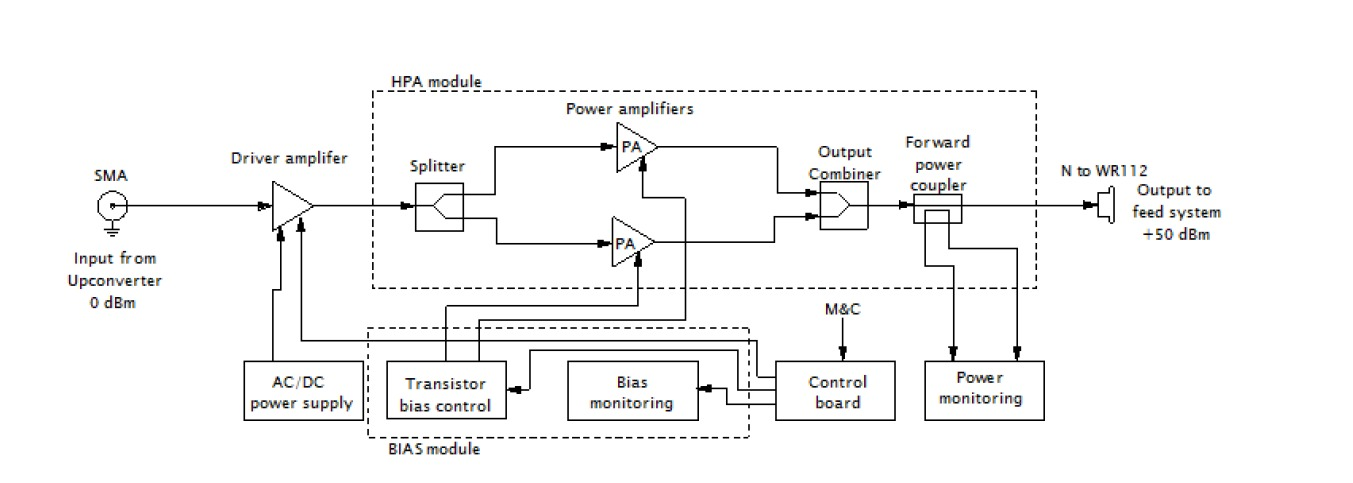
\includegraphics[width=0.9\textwidth]{bildes/HPA.jpg}\hspace{1cm}
    \caption{HPA augsta līmeņa blokshēma}
\end{figure}
(Informācija no M. Bleidera).
\subsection{Monitoringa sistēmas jaudas pastiprinātājiem}

\subsection{Aktīvā vidējā kvadrātiskā vērtības jaudas noteikana}
\chapter{X joslas raidīšanas sistēmas vadības bloka prototipa izstrāde}

Šajā nodaļā ir izklāstīta šī bakalaura darba ietvaros veiktā X joslas raidīšanas sistēmas vadības bloka prototipa izstrāde. Sākas nodaļa ar sistēmas pārskatu, tad tiek aprakstīts darba punkta iestatīšanas izstrādes process, kur tiek aprakstītas izveidotās iespiedplates, pēc kā tiek pievērsta uzmanība mikrokontrolierim, programmas kodam un lietojumprogrammas izstrādei, tad tiek aprakstīta jaudas monitorēšanas sistēmas izstrāde, kur beigās ir gala prototipu apraksts, kur tiek aprakstīts atsevišķo sistēmu novietojums korpusā. Visas izstrādnes, kas tika izstrādātas šī bakalaura ietvaros, tiek uzglabātas githubā\cite{bak_github}.

\section{RT-16 X-joslas raiduztverošās sistēmas pārskats}
Att 1.1. tiek parādīta X-joslas pārskats RT-16 radioteleskopam. Sistēmas vadība tiek veikta ar operatora jeb kontroles datoru, kas vada Cortex modemu \cite{cortex}, frekvenču lejuppārveidotāju un augšuppārveidotāju \cite{up_down_converters}, LNA un HPA. Cortex modēms paredzēts datu modulēšanai un demodulēšanai no satelīta. Frekvenču lejup un augšup pārveidotājs nepieciešams, lai varētu modulēto signālu pārnest uz nepieciešamo nesējfrekvenci noteiktam satelītam. HPA pastiprina modulēto signālu līdz 100 W (+50 dBm), lai palielinātu pārraides attālumu. HPA bloka pārraides jaudu noteica SSC. LNA nepieciešams, lai uzlabotu uztvertā signāla SNR un lai Cortex varētu to veiksmīgi demodulēt. Dipleksers un paraboliskā antena paredzēti signāla uztveršanai un pilna dupleksa komunikācijas nodrošināšanai.
\begin{figure}[H]
	\centering
    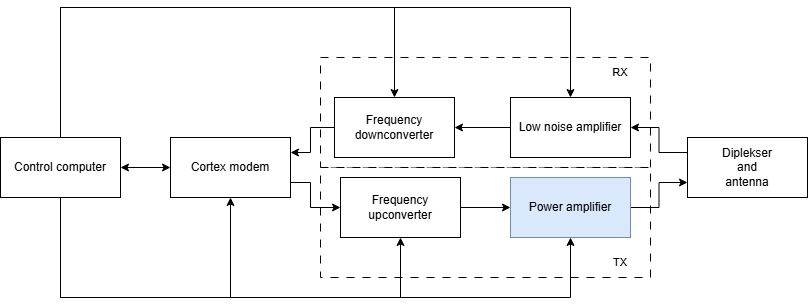
\includegraphics[width=\textwidth]{pictures/rt-16_x_diagram.jpg}\hspace{1cm}
    \caption{RT-16 X-joslas raiduztvērēja vispārīga bloka diagramma}
\end{figure}
Turpmāk darbā tiek apskatīts tikai augstas jaudas pastiprinātājs, kur daļa no tā tiek izstrādāta šī bakalaura ietvaros.
\section{Darba punkta nodrošināšanas sistēmas izstrāde}
Šajā nodaļā tiek aprakstīta izstrādes plates modifikācija un testēšana, izstrādātie līdzstrāvas sprieguma pārveidotāji, industriālā barošanas avota vadības, strāvas mērīšanas, ieslēgšanas/izslēgšanas elektriskā principiālā shēmas. Daļas, kas nodrošina darba punkta iestatīšanas/atiestatīšanas funkciju.
\subsection{Monitoringa izstrādes plates modifikācija un integrēšana}
Lai ātrāk iegūtu vēlamo rezultātu, tika iegādāta izstrādes plate ar izvēlēto monitorēšanas integrālo shēmu EVAL-AD7293 \cite{eval_board} ar AD piedāvātu vadības sistēmu EVAL-SDP-CB1Z \cite{eval_board_mcu}.
\begin{figure}[H]
	\centering
    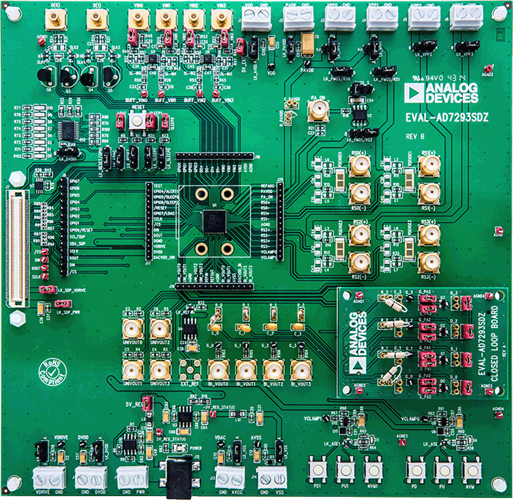
\includegraphics[width=0.5\textwidth]{pictures/EVAL-AD7293SDZ_TOP-web.png}\hspace{1cm}
    \caption{AD7293 izstrādes plate}
\end{figure}
\begin{figure}[H]
	\centering
    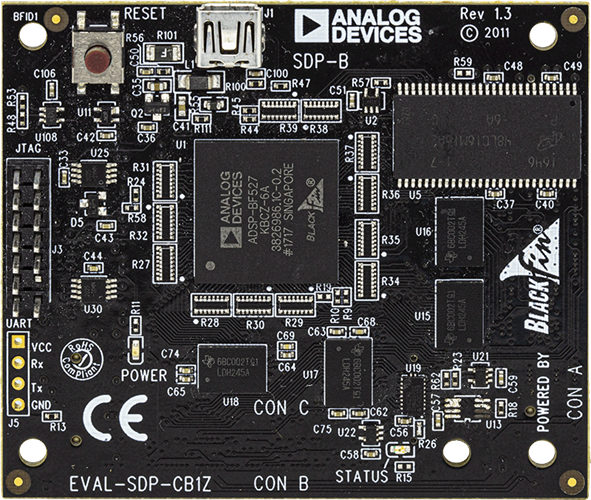
\includegraphics[width=0.5\textwidth]{pictures/EVAL-SDP-B-top-web.png}\hspace{1cm}
    \caption{Vadības sistēma monitorēšanas izstrādes platei}
\end{figure}
Šīs sistēmas pārbaudei tika izmantota AD lietojumprogramma, kas sniedz vispārīgu pārskatu par sistēmas funkcionalitāti.
\begin{figure}[H]
	\centering
    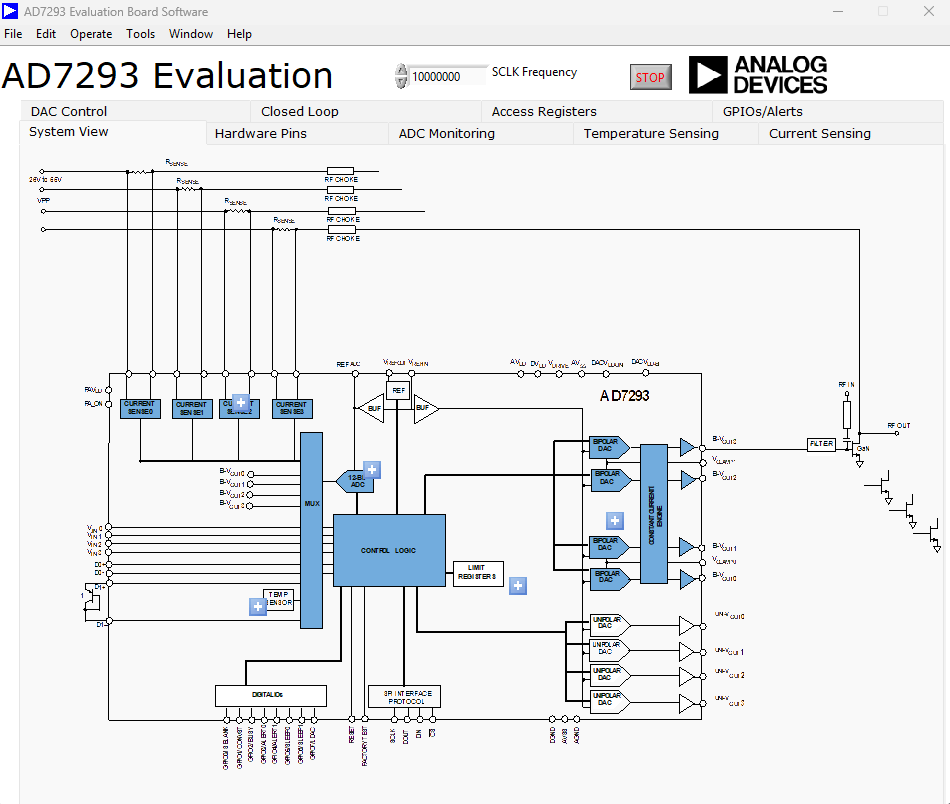
\includegraphics[width=0.6\textwidth]{pictures/eval-soft.png}\hspace{1cm}
    \caption{AD7293 testēšanas lietojumprogramma}
\end{figure}
Sekojot datu lapā pieejamai informācijai tika nodrošināta reģistru konfigurācijas secība un sasniegta vēlamā funkcionalitāte darba punkta iestatīšanai un atiestatīšanai.\\
Pēc nepieciešamās funkcionalitātes nodrošināšanas tika veiktas izstrādes plates modifikācijas - atlodēti SMA konektori, lai varētu pielodēt strāvas monitorēšanas sistēmas izvadus un ieslēgšanas/izslēgšanas sistēmas vadības izvadu, samainīti savienotājelementi, pievienoti barošanas avoti un pievienots digitālās loģikas analizators, lai monitorētu SPI saskarni.
\begin{figure}[H]
	\centering
    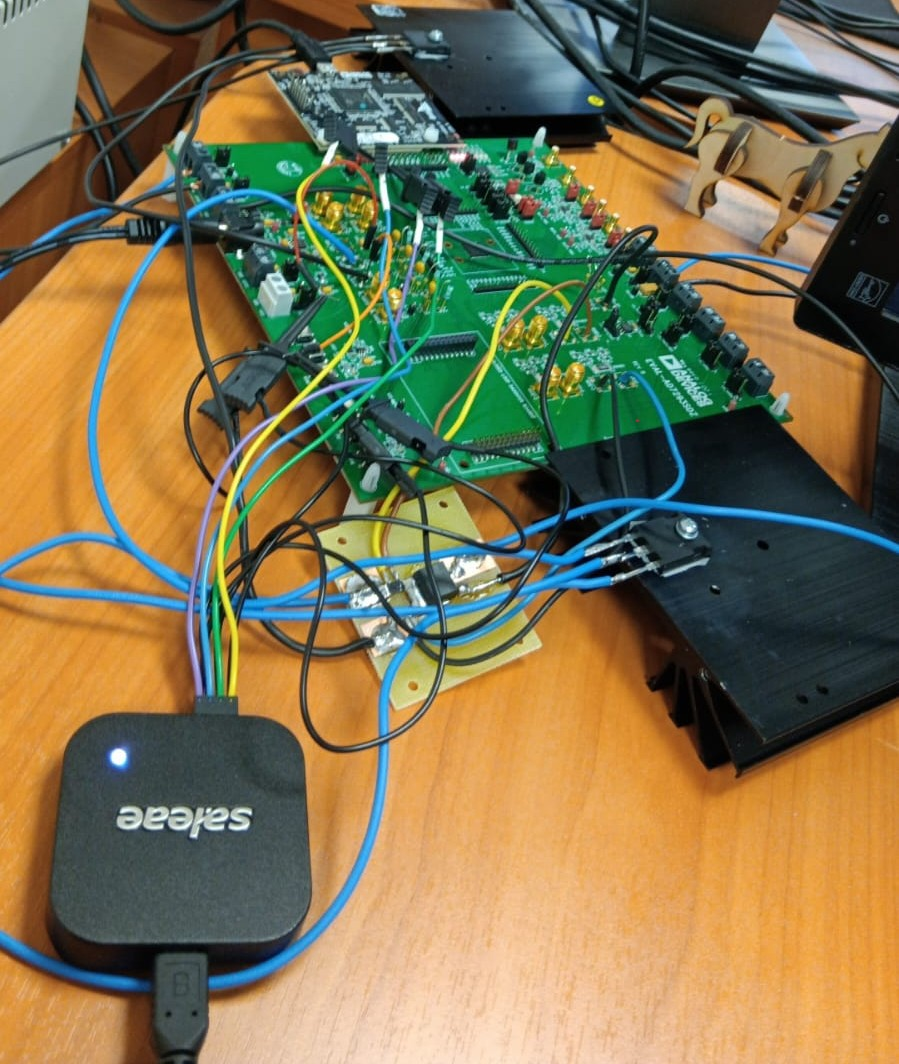
\includegraphics[width=0.5\textwidth]{pictures/daf.jpg}\hspace{1cm}
    \caption{Testa stends ar testa lauktranzistoriem}
\end{figure}
Tad tika sasniegts vēlamais rezultāts ar darba punkta iestatīšanu un atiestatīšanu.
\subsection{Sprieguma pārveidotāji, temperatūras sensora un 24 V barošanas avota vadības shēmas}
Tika izvēlēti lineārie sprieguma stabilizatori 5 un 9 V līnijām, neskatoties uz zemo efektivitāti, salīdzinot ar impulsa tipa sprieguma stabilizatoriem, tie nerada trokšņus izejā. Lineārie sprieguma stabilizatori tiek slēgti virknē, lai palielinātu 5 V regulātora efektivitāti, samazinot sprieguma kritumu uz tā. 12 V tiek pārveidots uz 9 V un no 9 V tiek pārveidots uz 5 V.  
\begin{figure}[H]
	\centering
    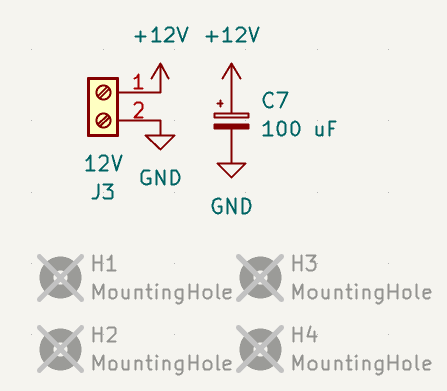
\includegraphics[width=0.6\textwidth]{pictures/inputs.png}\hspace{1cm}
    \caption{Ievadi, elektrolītiskais kondesators un urbjcaurumi}
\end{figure}
J3 terminālbloks ir paredzēts, lai varētu pieslēgt industriālo 12 V barošanas avotu. C7 elektrolītiskais kondensators paredzēts, lai mazinātu ieejas pulsācijas. H1, H2, H3 un H4 urbjcaurumi paredzēti, lai iespiedplati varētu iestiprināt korpusā.
\begin{figure}[H]
	\centering
    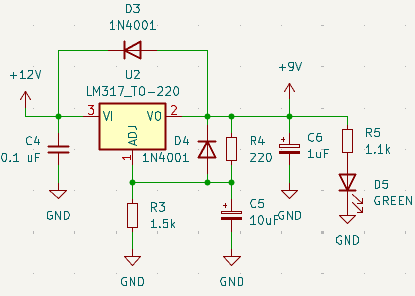
\includegraphics[width=0.6\textwidth]{pictures/9v.png}\hspace{1cm}
    \caption{12 V uz 9 V pārveidotais}
\end{figure}
\begin{figure}[H]
	\centering
    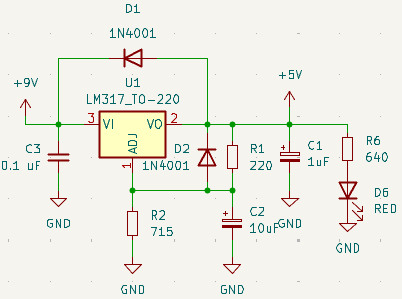
\includegraphics[width=0.6\textwidth]{pictures/5v.png}\hspace{1cm}
    \caption{9 V uz 5 V pārveidotais}
\end{figure}
Sprieguma iestatīšanai tiek izmantota atgriezeniskā saite, ko veido rezistori R1, R2, R3 un R4. Ķēdē tiek izmantoti keramiskie kondensatori C1, C3, C4 un C6. keramiskie un elektrolītiskie kondensatori ir vajadzīgi, lai mazinātu barošanas pulsācijas. R6 un R5 ir strāvas ierobežojošie rezistori D5 un D6 gaismas diodēm. D1, D2, D3 un D4 taisngriežu diodes paredzētas, lai neļautu C2 un C5 kondensatoriem izlādēties lineārā sprieguma izejā.
\begin{figure}[H]
	\centering
    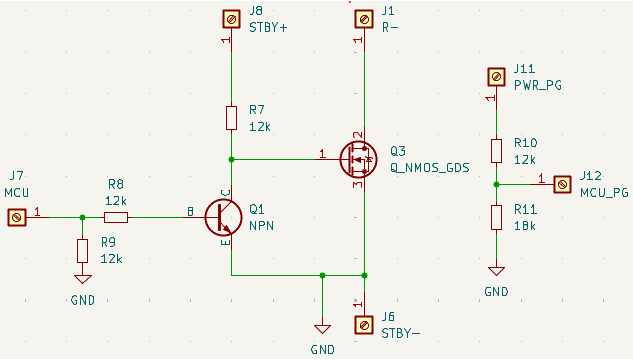
\includegraphics[width=0.6\textwidth]{pictures/24_control_detection.png}\hspace{1cm}
    \caption{24 V barošanas avota vadības sistēmu}
\end{figure}
J7 izvads paredzēts, lai varētu pieslēgt mikrokontrolliera vadības signālu. R8 ir paredzēts strāvas ierobežošanai NPN bipolārajam tranzistoram. R9 ir zema līmeņa piesaistes rezistors, lai pārejas procesā netiktu atvērts tranzistors. R7 rezistors ir paredzēts strāvas ierobežošanai un augsta signāla līmeņa piesaistei pie N kanāla lauktranzistora aizvara. J8, J1 un J6 izvadi paredzēti, lai varētu vadīt 24 V industriālo barošanas avotu. J11 ir paredzēts barošanas avota stāvokļa pieslēgvieta, kur R10 un R11 rezistori ir sprieguma dalītāji, lai varētu veikt sprieguma nolasi ar mikrokontrolliera.
\begin{figure}[H]
	\centering
    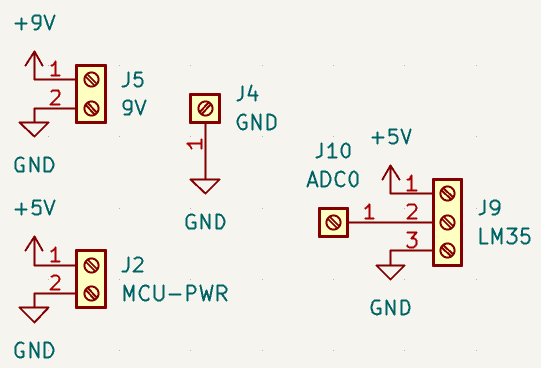
\includegraphics[width=0.6\textwidth]{pictures/outputs.png}\hspace{1cm}
    \caption{Pieslēgvietas MCU, temperatūras un patērētājiem}
\end{figure}
J5 un J2 terminālbloks paredzēts, lai varētu nodrošināt 9 V un 5 V barošanu patērētājiem. J9 terminālbloks paredzēts temperatūras sensora pieslēgšanai. J10 ir izvads, paredzēts mikrokontroliera ADC pieslēgvietai.
\begin{figure}[H]
	\centering
    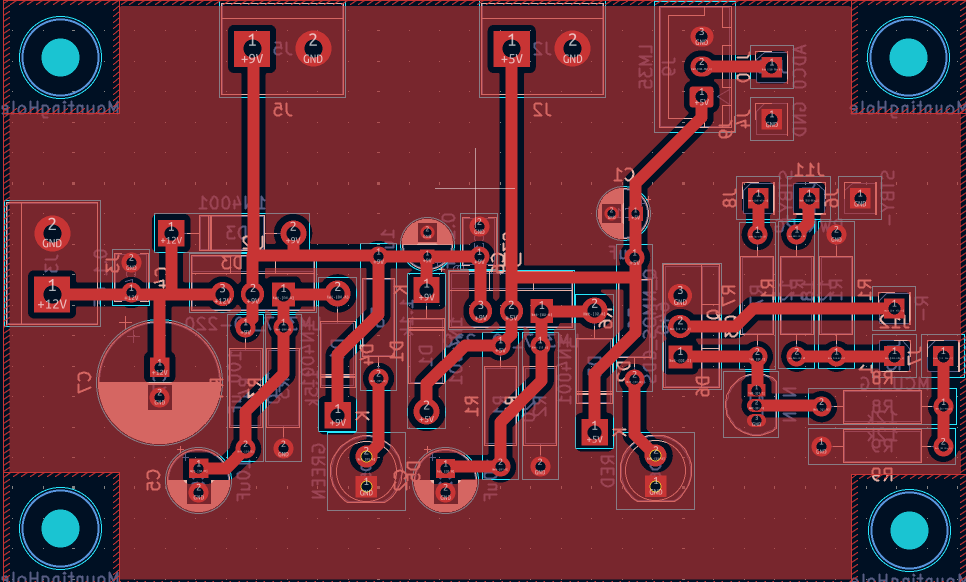
\includegraphics[width=0.6\textwidth]{pictures/power_board.png}\hspace{1cm}
    \caption{Iespiedplate lietojumprogrammatūrā "KiCad"}
\end{figure}
 Iespiedplate tika trasēta vienā slānī. Komponentes tika izvietotas pēc iespējas blīvāk, lai samazinātu iespiedplates izmērus. Tika izmantotas THT komponentes. Iespiedplate tika izfrēzēta ar augstskolā pieejamo frēzi.
\subsection{Strāvas mērīšanas iespiedplate ar ieslēgšanas/izslēgšanas slēdzi}
\begin{figure}[H]
	\centering
    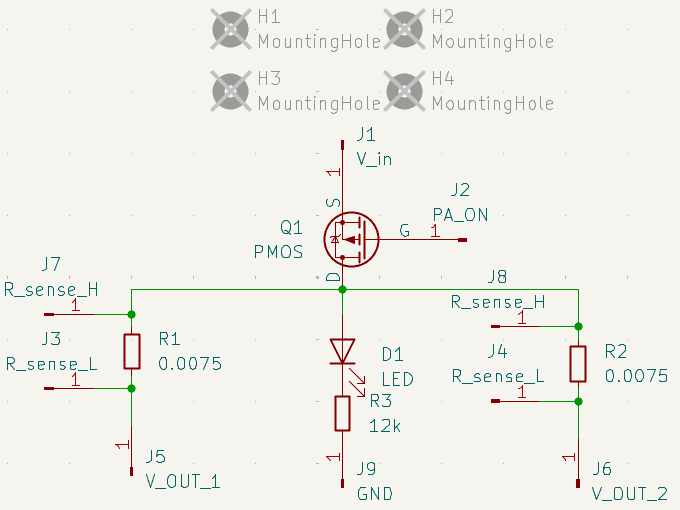
\includegraphics[width=0.6\textwidth]{pictures/shunt_resistors.png}\hspace{1cm}
    \caption{Strāvas mērīšanas shematiskais zīmējums}
\end{figure}
J1 terminālbloks ir 24 V pieslēgvietas nodrošināšanai. Q1 P kanāla lauktranzistors tiek izmantots slēdža režīmā, kas tiek kontrolēts ar AD7293 monitorēšanas integrālo shēmu, kas tiek pievadīts caur J2 termināli. R1 un R2 ir šunta rezistori strāvas mērīšanai. Šunta rezistori tika aprēķināti pēc izvēlētā mērīšanas diapazona AD7293 un maksimālās strāvas R <= 0.025/3 . J3, J4, J7 un J8 izvadi ir paredzēti, lai pieslēgtu strāvas mērīšanas sistēmu. D1 gaismas diodē ir paredzēta sistēmas stāvokļa identificēšanai. R3 rezistors ir paredzēts strāvas ierobežošanai, lai pasargātu gaismas diodi. J9 izvads paredzēts zemējuma nodrošināšanai.
\begin{figure}[H]
	\centering
    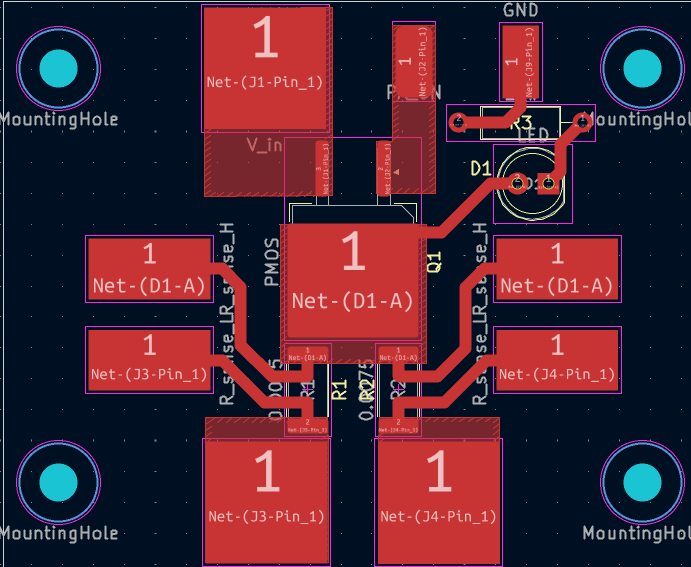
\includegraphics[width=0.6\textwidth]{pictures/shunt_resistors_board.png}\hspace{1cm}
    \caption{Iespiedplate lietojumprogrammatūrā "KiCad"}
\end{figure}
Tika izstrādāta vienslāņu plate ar blīvu komponenšu izvietojumu un attiecīgu jaudas celiņu platumiem. Tā tika izfrēzēta ar VeA pieejamo frēzi.

\section{Mikrokontroliers un vadības sistēma caur tīklu}
Kā mikrokontrolieris tika izvēlēts W5500-EVB-Pico \cite{pico}, balstoties uz darba vadītāja ieteikumu, kam ir TCP/IP tīkla steka atbalsts, ar kuru ir gatavi TCP servera piemēri, kas saņem un nosūta komandas tīklā, kā arī mikrokontrolierim ir divi kodoli.
\begin{figure}[H]
	\centering
    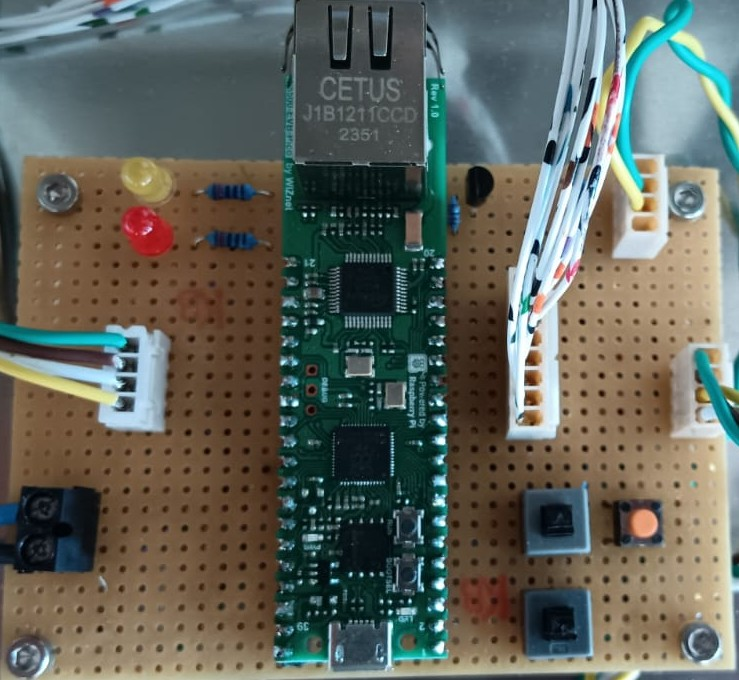
\includegraphics[width=0.6\textwidth]{pictures/mcu_board.jpg}\hspace{1cm}
    \caption{Mikrokontroliera iespiedplate}
\end{figure}
RP4020 mikrokontrolieris tiek plaši pielietots iegultajās sistēmās, jo viena mikroshēma satur CPU, atmiņu, RAM, watchdogs u.c. perifērijas. Tika izvēlēts Arduino IDE šim mikrokontrolierim, izmantojot C un C++ programmēšanas valodas. Arduino vide tika izvēlēta dēļ gatavo bibliotēku pieejamības WS5500 tīkla modulim \cite{ws5500}, un VSRC izstrāde ir balstīta uz šīm bibliotēkām.
\begin{figure}[H]
	\centering
    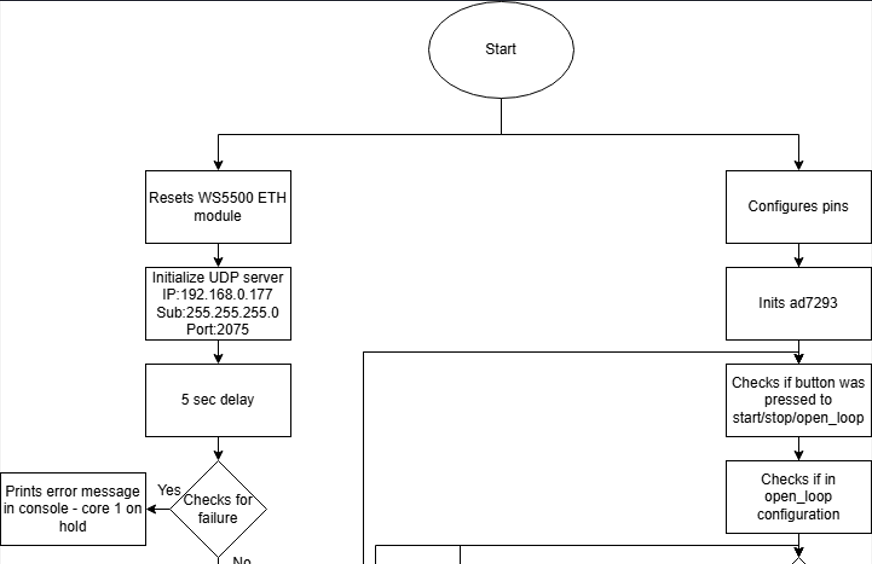
\includegraphics[width=0.8\textwidth]{pictures/prog_code_1.png}\hspace{1cm}
    \caption{Daļa no programmas koda bloka diagramma}
\end{figure}
Divkodolu mikrokontrolierim tiek izmantots viens kodols servera uzturēšanai un datu pārraidei, bet otrā tiek kontrolēti mikrokontroliera izvadi, monitorēšanas integrālā shēma, temperatūras mērīšana un sistēmas statusa noteikšana. Programmas kods sākas ar to, ka pirmajā kodolā tiek restartēts un konfigurēts WS5500 modulis, tad tiek konfigurēts izvadīts kļūdas paziņojums, tas tiek darīts 3 reizes un pēc trešās reizes, ja nesanāk, tad kodols tiek apstādināts. Otrā kodolā nokonfigurē izvadus un darba punkta un monitorēšanas integrālo shēmu. Tad tiek pārbaudīts, vai ir nospiesta viena no trim pogām. Spiedpogas paredzētas manuālai testēšanai, kur pirmā spiedpoga atbild par sistēmas ieslēgšanu un darba punkta nodrošināšanu, otrā spiedpoga nodrošina sistēmas izslēgšanu un darba punkta atiestatīšanu, bet trešā, lai deaktivizētu slēgto ciklu, lai varētu pārraidīt RF signālu ar mainīgu jaudu. Tiek pārbaudīts, vai ir atvērtā cikla konfigurācijā, ja jā, tad tiek aktivizēta gaismas diode, kas atrodas uz mikrokontroliera plates.
\begin{figure}[H]
	\centering
    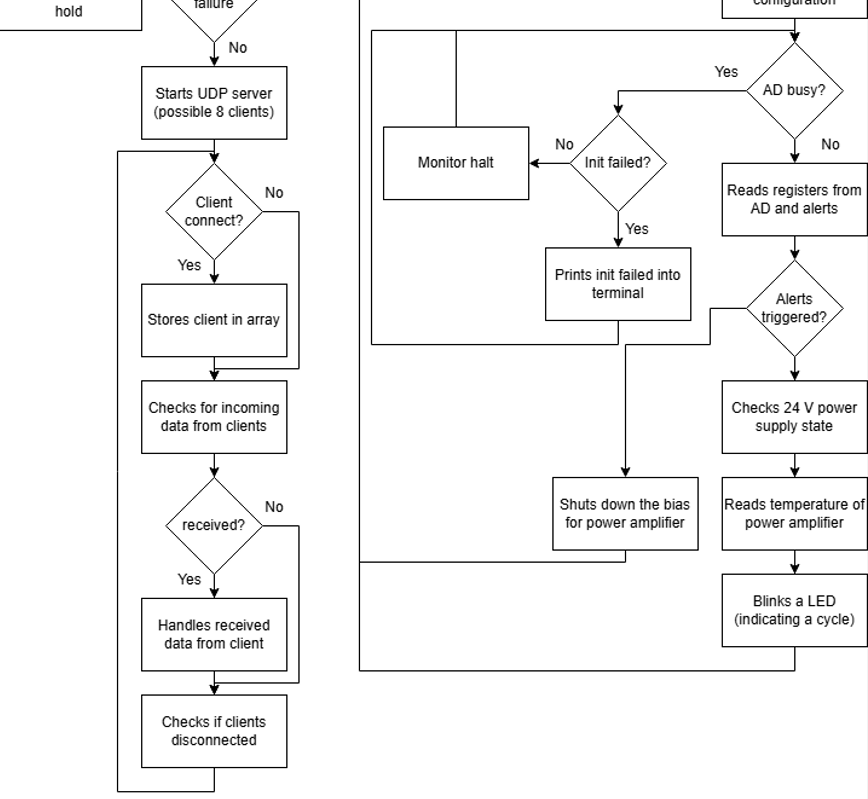
\includegraphics[width=0.8\textwidth]{pictures/prog_code_2.png}\hspace{1cm}
    \caption{Daļa no programmas koda bloka diagramma}
\end{figure}
Pirmajā kodolā tiek uzsākts serveris, pie kura var pieslēgties līdz astoņiem klientiem. Pirmajā kodolā tiek pārbaudīts, vai ir jauns klienta pieslēgšanās pieprasījums, ja ir, tad klienta TCP objektu saglabā masīvā, kas glabā informāciju par klienta IP adresi un portu, kā arī savienojuma stāvokli, bet, ja nav, tad pārbauda, vai ir saņemti komandas no klientiem, ja tādi ir, ja kādi dati ir saņemti, tad to apstrādā un veic attiecīgu darbību, bet, ja nav, tad pārbauda, vai kāds klients ir atslēdzies no servera, lai varētu atbrīvot masīvu un vietu citam klientam. Otrā kodolā tiek pārbaudīts, vai monitorēšanas integrālā shēma ir aizņemta, tas datu lapā netiek uzsvērts, bet pārbaude netraucē, ja ir, tad pārbauda, vai tā tiek izmantota citā procesā vai ir inicializācijas problēmas, tad pārbauda tās statusu atkal. Ja AD7293 ir gatavs komunikācijai, tad tiek nolasīti reģistri un karodziņi, ja kāds no karodziņiem tiek aktivizēts, tad darba punktu atiestata un atslēdz sistēmu, bet, ja nav, tad tiek pārbaudīts 24 V elektrobarošanas statuss, nolasīta temperatūra un ieslēdz un ar aizskavi izslēdz gaismas diodi, kas atspoguļo viena cikla beigas.\\
Mikrokontrolieris saglabā sistēmas esošo stāvokli mainīgajā, nolasa datus no sensoriem un monitorēšanas integrālās shēmas datus, kuri tiek strukturizēti simbolu virknē un nosūtīti caur TCP protokolu klientam pēc pieprasījuma. Zemāk apkopota telemetrijas virkne.
\begin{table}[H]
\centering
\captionsetup{singlelinecheck=off, justification=raggedleft}
\caption{Telemetrijas virknes struktūra un atšifrējums}
\renewcommand{\arraystretch}{1.2}
\begin{tabular}{|c|c|l|l|}
\hline
\multirow{24}{*}{\centering 96 baiti} & \textbf{Datu tips} & \textbf{Mainīgā nosaukums} & \textbf{Definīcija} \\
\hline
\cline{2-4}
& I    & pa\_on\_state          & HPA stāvoklis (0=off, 1=on) \\
\cline{2-4}
& I    & psu\_pg\_state         & Barošanas avota status (0=off, 1=on) \\
\cline{2-4}
& I    & open\_loop\_mode       & Kontroles režīms (0=closed, 1=open) \\
\cline{2-4}
& F    & rs0\_volts            & Noteces spriegums HPA \\
\cline{2-4}
& UI   & rs\_alert\_high       & Maksimālā noteces slieksņa brīdinājums\\
\cline{2-4}
& UI   & rs\_alert\_low        & Minimālā noteces slieksņa brīdinājums\\
\cline{2-4}
& UI   & alert0\_state         & Sistēmas brīdinājumu status \\
\cline{2-4}
& F    & isense0\_amps         & Strāvas mērījums 0 kanālam\\
\cline{2-4}
& F    & isense1\_amps         & Strāvas mērījums 1 kanālam\\
\cline{2-4}
& F    & Ug0\_volts            & Aizvara sprieguma 0 mērījums \\
\cline{2-4}
& F    & Ug0\_volts\_lim       & Aizvara sprieguma 0 limits \\
\cline{2-4}
& F    & Ug1\_volts            & Aizvara sprieguma 1 mērījums \\
\cline{2-4}
& F    & Ug1\_volts\_lim       & Aizvara sprieguma 1 limits \\
\cline{2-4}
& F    & temp\_degC            & Temperatūra korpusā \\
\cline{2-4}
& F    & temp1\_degC           & Temperatūra uz HPA 1 \\
\cline{2-4}
& F    & temp2\_degC           & Temperatūra uz HPA 2 \\
\cline{2-4}
& F    & temp\_degC\_Fpwr      & Izstarotā jaudas mērītāja temperatūra \\
\cline{2-4}
& F    & temp\_degC\_Rpwr      & Atstarotās jaudas mērītāja temperatūra\\
\cline{2-4}
& F    & temp\_degC\_AD7293      & Monitorēšanas IC temperatūra\\
\cline{2-4}
& F    & reflected\_power\_log      & Atstarotā jauda dBm \\
\cline{2-4}
& F    & reflected\_power\      & Atstarotā jauda W\\
\cline{2-4}
& F    & forward\_power\_log        & Izstarotā jaudas dBm \\
\cline{2-4}
& F    & forward\_power\        & Izstarotā jaudas W \\
\cline{2-4}
& F    & $S_{11}$\_param\        & Izstarotā jaudas W \\
\hline
\end{tabular}
\end{table}
 Struktūra sastāv no 96 baitiem. Pirmie 4 baiti satur esošo jaudas pastiprinātāja stāvokli (izslēgts, ieslēgts), otrie 4 baiti satur 24 V elektrobarošanas statusu (ieslēgts, izslēgts), trešie 4 baiti satur informāciju par to, vai ir cikla konfigurācijā, ceturtie 4 baiti, kas atgriež sprieguma kritumu uz šunta rezistora, tad nākošie 4 baiti atgriež karodziņu vecāko un jaunāko baitu, tad nākošie četri ir karodziņi. Isens0 atgriež strāvas vērtību caur pirmo šunta rezistoru, kur Isense1 atgriež strāvas vērtību caur otro šunta rezistoru. Tālāk iet UG0 volti, kas nosaka, kāds ir aizvara vadības sprieguma līmenis pirmajam pastiprinātājam, tad ir ierobežojums, kas nosaka iestatītās robežvērtības, tad nākošie 8 baiti nozīme ir ekvivalenta tikai otram pastiprinātājam. Nākošie 4 baiti ir temperatūras mērījums korpusā, tad 8 baiti ir temperatūras mērījumi divos punktos uz jaudas pastiprinātāja, tad nākošie 8 baiti ir jaudas mērītāju IC temperatūra izstarotajai un atstarotajai jaudai un 4 baiti monitorēšanas IC temperatūra. Nākošie 16 baiti ir izstarotās un atstarotās jaudas logaritmiskā un matemātiskā reprezentācijā. Pēdējais ir S11 parametrs.\\
 Klients var nosūtīt vairākas komandas mikrokontrolierim, lai iestatītu režīmu, mainītu konfigurāciju un pieprasītu datus.
 \begin{table}[H]
\centering
\captionsetup{singlelinecheck=off, justification=raggedleft}
\caption{Iespējamās komandas un to atšifrējums}
\renewcommand{\arraystretch}{1.2}
\begin{tabular}{|c|c|l|l|}
\hline
\multirow{6}{*}{\centering 15 baiti} & \textbf{Datu tips} & \textbf{Mainīgā nosaukums} & \textbf{Definīcija} \\
\hline
\cline{2-4}
& S    & mon          & Pieprasa telemetrijas virkni \\
\cline{2-4}
& S    & pon          & Aktivizē/deaktivizē sistēmu \\
\cline{2-4}
& S    & olm          & Maina noslēgtās cilpas konfigurāciju \\
\cline{2-4}
& S    & setcurr          & Iestata noteces strāvu kanāliem \\
\cline{2-4}
& S    & setramp          & Iestata darba punkta iestatīšanas periodu \\
\hline
\end{tabular}
\end{table}
Maksimālā simbola virkne, ko var apstrādāt mikrokontrolieris, ir 15 baiti. Mon komanda ir vienīgā, kura nepieņem papildus argumentus, mikrokontrolieris saņemot šo komandu, atbild nekavējoties ar telemetrijas virkni klientam. Pon komanda pieņem vienu argumentu 0 vai 1, ja tiek saņemts 1, tad tiek uzsākta sistēmas darbība (elektrobarošanas ieslēgšana, darba punkta nodrošināšana u.c.), bet, ja saņem 0, tad sistēmas darbība tiek pārtraukta (darba punkta atiestatīšana, elektrobarošanas izslēgšana u.c.). Olm komanda pieņem vienu argumentu 0 vai 1, ja saņemts ir 1, tad slēgtais cikls tiek izslēgts, ja saņem 0, tad to aktivizē. Ja tiek padoti nepareizi ieejas argumenti, tad sistēma atbild ar iespējamajiem variantiem lietotājam. Setcurr komanda pieņem peldošā komata mainīgo, kas iestata darba punkta strāvu visiem kanāliem. Setramp pieņem float argumentu, ar kuru var izmainīt darba punkta noturēšanas strāvu no 250~\textmu s līdz 31.75~ms
\begin{figure}[H]
	\centering
    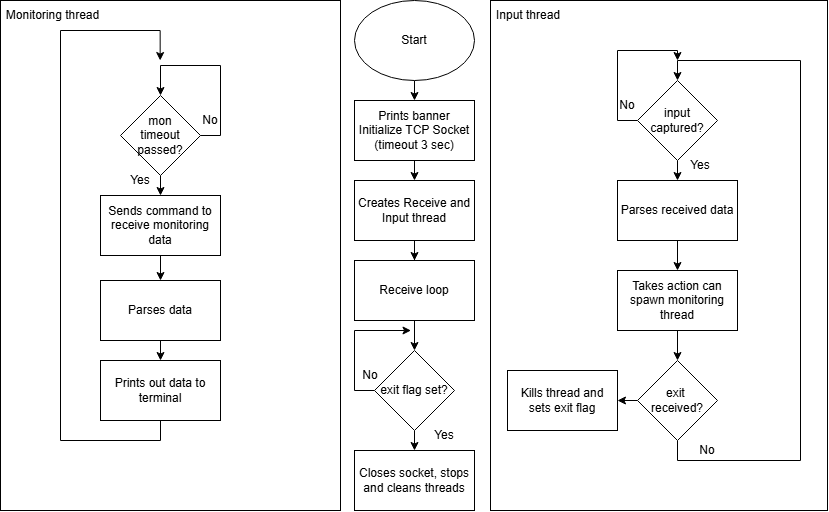
\includegraphics[width=0.8\textwidth]{pictures/script_program.drawio.png}\hspace{1cm}
    \caption{Python skripta bloka diagramma}
\end{figure}
Tika izveidots Python skripts uz Windows 11 OS, kas uzsāk X-joslas sistēmas darbību. Skriptu startējot, tiek terminālī izvadīts logo, atšifrējums, sistēmas nosaukums un palīginstrukcija ar visām iespējamām darbībām. Tad tiek izveidots TCP klients, kurš mēģina pieslēgties pie TCP servera ar 3 sekunžu intervālu; ja neizdodas, skripts beidz savu darbu. Kad ir izveidots savienojums ar serveri, tad skripts izveido ievades pavedienu un ieiet uztveršanas ciklā. Uztveršanas cikls gaida ienākošo simbolu virkni un saņemšanas brīdī to izvada; ja nekas netiek saņemts, tad tiek izvadīts paziņojums, ka serveris ir pārtraucis kontaktēties, un beidzas skripta darbība. Ievades pavedienā tiek termināli izvadīts teksts ar aicinājumu uzsākt sistēmas darbību ar "start", kas uzsāk X-joslas sistēmas darbību, aktivizējot sistēmu un iestatot darba punktu ar noklusējuma vērtībām. Kad tiek saņemta simbolu virkne, tā tiek pārbaudīta, vai virkne atbilst kādai no iespējamajām funkcijām; ja nē, tas tiek automātiski nosūtīts mikrokontrolierim. Ja komanda atbilst kādai no skripta funkcionalitātēm, tad tā tiek parsēta un attiecīgi izvadīta informācija vai pārtraukta tās darbība. Kad tiek nosūtīta start komanda, skripts izveido monitorēšanas pavedienu, kur ik pēc iestatītā intervāla tiek veikta telemetrijas virknes nolase no mikrokontroliera, tad ienākošā telemetrija tiek parsēta un izvadīta lietotājam ērtākā virtenē. Ja tiek saņemta "exit" komanda vai ctrl+c kombinācija, tad automātiski sistēma pārtrauc savu darbību un pārbauda, vai kāds no pavedieniem ir aktīvs; ja ir, tad to pārtrauc, kā arī tiek pārbaudīts sistēmas stāvoklis; ja tas ir ieslēgts, tad to izslēdz pirms skripts aizveras.
\section{Jaudas detektora izstrāde}
Ir divas jaudas mērīšanas integrālās shēmas, kas veic atstarotās un izstarotās jaudas mērīšanu. R8 rezistors tiek izmantots, lai salāgotu ievades pretestību. C12 un C11 veido augstfrekvenču filtru un tam jābūt tādam, lai netiktu nogriezta 7.2 GHz frekvence. C10 keramiskais kondensators paredzēts vidējošanas funkcijas iekšējai RMS aprēķināšanai. Lai kompensētu temperatūras dreifēšanu, tiek izmantoti R6 un R7 rezistori pēc datu lapas ieteikumiem Rf signālam virs 5.8 GHz. R9 un R10 rezistori veido sprieguma dalītāju, lai panāktu 0.8 V uz VTGT, kas veido kompromisu starp precizitāti un maksimālu dinamisko diapozonu. C8, C9, C13 un C14 ir barošanas filtri. J8 ir SMA konektors, lai pieslēgtu mērāmo signālu.
\begin{figure}[H]
	\centering
    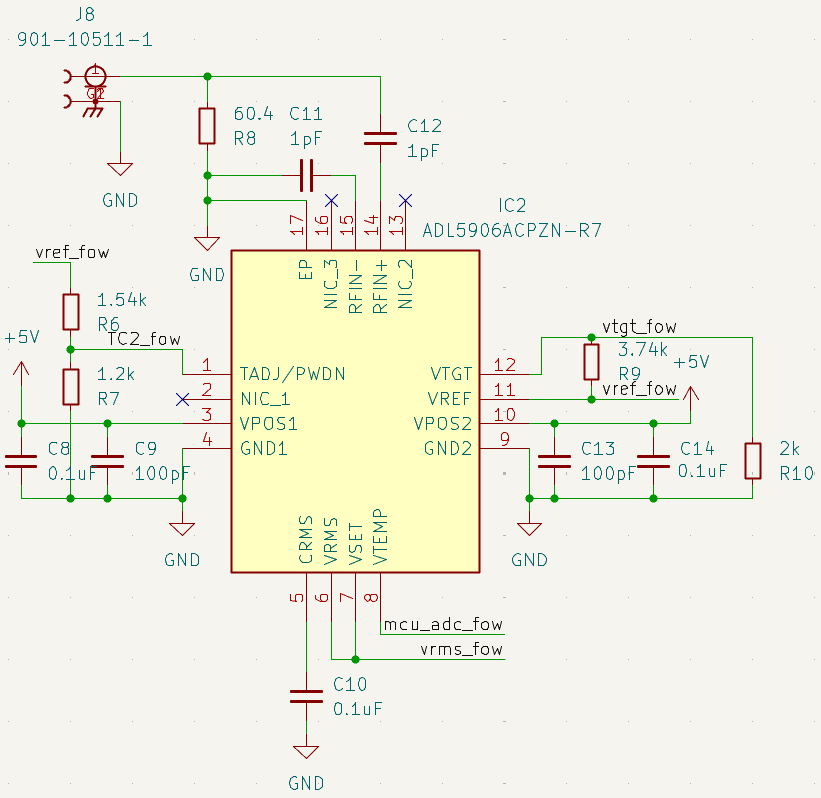
\includegraphics[width=0.5\textwidth]{pictures/fwd_powerdetector.png}\hspace{1cm}
    \caption{Jaudas noteikšanas integrālā shēma}
\end{figure}
Tika izveidota četru slāņu plate. Iespiedplates izstrādē liels uzsvars tika veikts uz pāris komponenšu izvēli, kondensatoru rezonanses frekvencei bija jābūt augstākai par mērāmo, celiņa platumam ieejā bija jābūt tādam, lai trakts būtu salāgots ar 50 ohm pretestību, SMA konektora kontaktlaukuma izmērs nedrīkstēja pārsniegt celiņa platumu, lai neveidotos signāla atstarojumi savienojuma vietā. Komponentes tika novietotas pēc iespējas tuvāk integrālajai shēmai, lai atbrīvotos no liekas parazītiskās induktivitātes. Trasējums veikts pēc datu lapas ieteikuma. 
\begin{figure}[H]
	\centering
    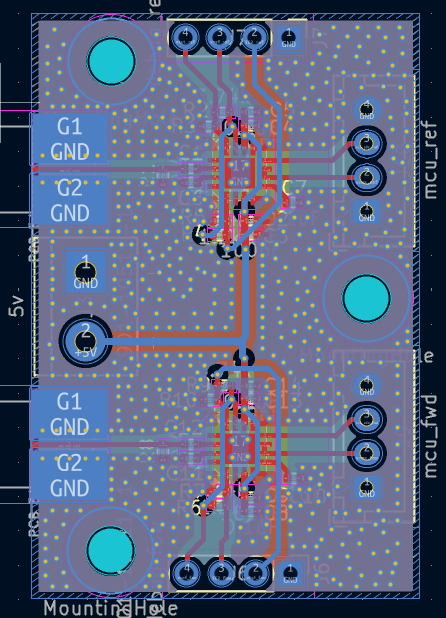
\includegraphics[width=0.6\textwidth]{pictures/board_powerdetector.png}\hspace{1cm}
    \caption{Jaudas noteikšanas iespiedplate}
\end{figure}

\subsection{Gala prototips}
1. pozīcijā ir HPA un uz viņa novietotie testa lauktranzistori, kas simulē jaudas pastiprinātājus. 2. pozīcijā ir līniju iezīmētie industriālie barošanas avoti. 3. pozīcijā ir monitorēšanas izstrādes plate. 4. pozīcijā ir mikrokontroliera plate. 5. pozīcijā ir RMS jaudas mērītājs. 6. pozīcijā ir pārveidotāju un barošanas avota vadības shēma. 7. pozīcija ir ieslēgšanas/izslēgšanas shēma ar strāvas mērīšanu. 
\begin{figure}[H]
	\centering
    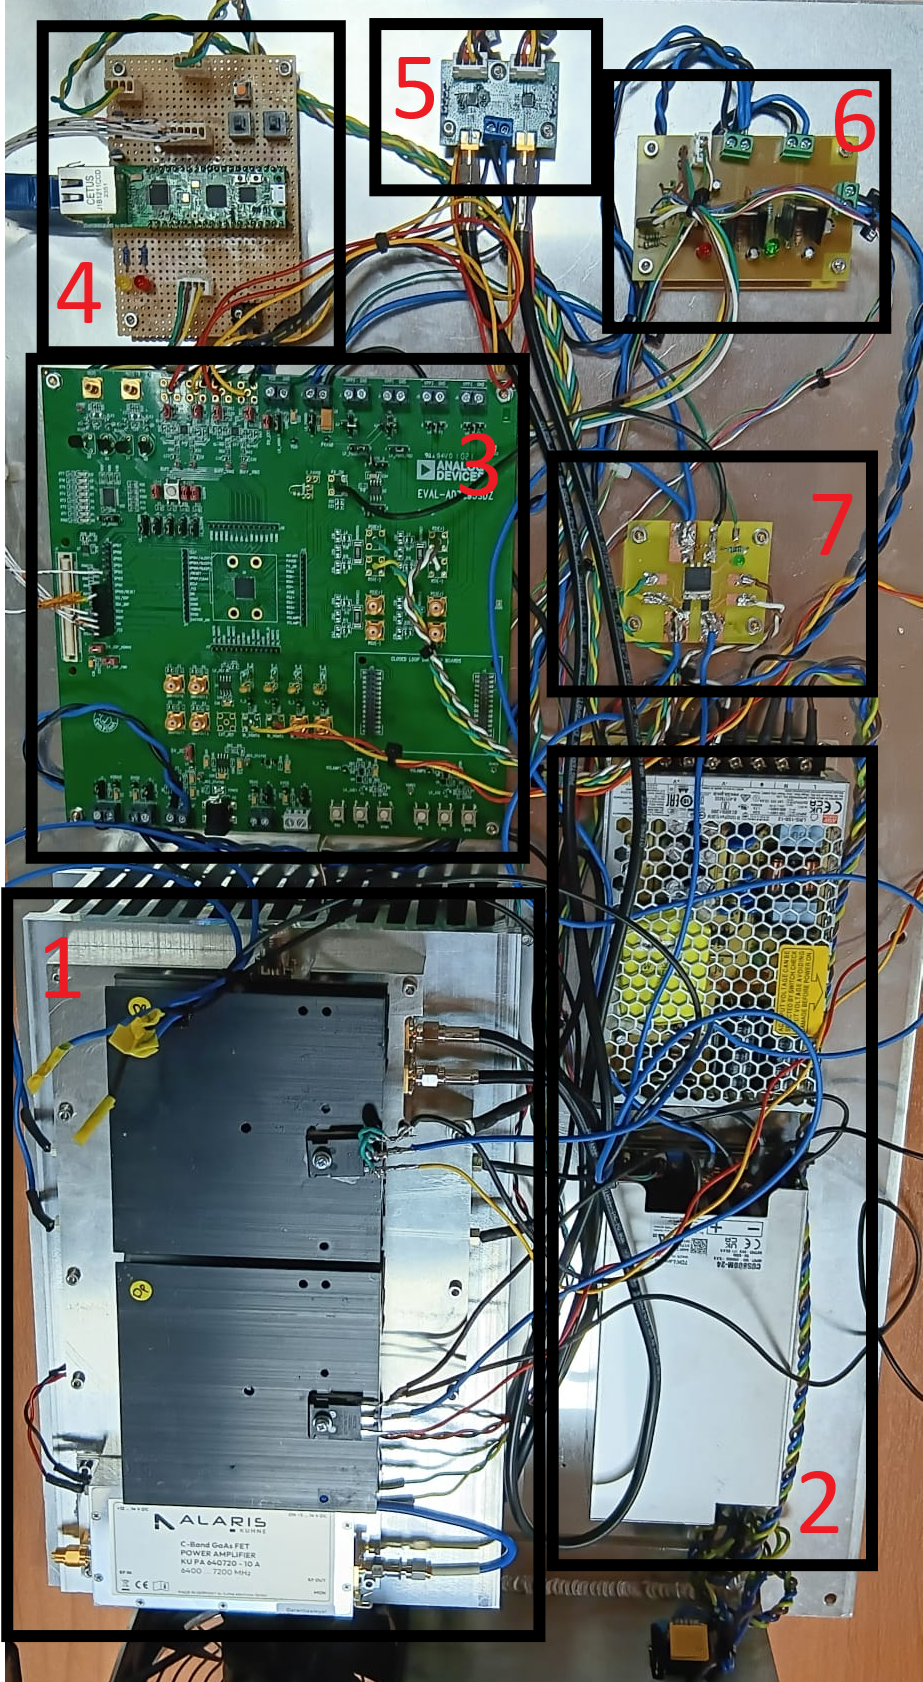
\includegraphics[width=0.9\textwidth]{pictures/finished.png}\hspace{1cm}
    \caption{Prototipa stends}
\end{figure}
\chapter{Testi}
Testi tika sadalīti vairākās daļās, lai pārliecinātos par atsevišķu apakšsistēmu funkcionalitāti. Visi testi izriet no specifikācijas, lai pārbaudītu sistēmu atbilstību. Testi ietver darba punkta iestatīšanu RF jaudas pastiprinātājam, digitālās loģikas barošanas risinājuma novērtējumu, jaudas detektora elektrisko parametru noteikšanu pie 7.2 GHz un tīkla vadību ar TCP protokolu. Testos tiek izmantotas tādas mēriekārtas kā Metex M-3604D digitālais rokas multimetrs \cite{metex_multimeter}, Fluke 87 digitālais multimetrs \cite{fluke_multimeter}, SIGLENT SDS-1104X-U osciloskops \cite{oscil}, Rohde\&Schwarz signāla ģenerators SMP04 \cite{rs_signal_generator}, Rohde\&Schwarz VNA ZVK \cite{rs_vna}, BaseTech BT-305 barošanas avots \cite{test_powersupply} un IGENT SPL 1020 XE 200W DC programmējamo slodzi \cite{programmable_load}.
Testa sadaļās:
\begin{itemize}
    \item Darba punkta iestatīšanas/attiestatīšanas.
    \item 5 un 9 V barošanas risinājuma novērtējums.
    \item Jaudas detektora un koaksiāļo kabeļu novērtējums.
    \item Sistēmas vadība caur tīklu.
\end{itemize}

\section{HPA darba punkta iestatīšana/atiestatīšana}
Darba punkta noteikšanai (skat. 3.1. att.) tika mērīta noteces strāva , 12  un 24 V industriālā barošanas avota līnijas, ieslēgšanas/izslēgšanas slēdža vadības signāls un RF jaudas pastiprinātāja aizvara spriegums. Noteces strāva jaudas pastiprinātājam tiek mērīta ar multimetru, bet pārējie sistēmas parametri - ar osciloskopu.
\begin{figure}[H]
	\centering
    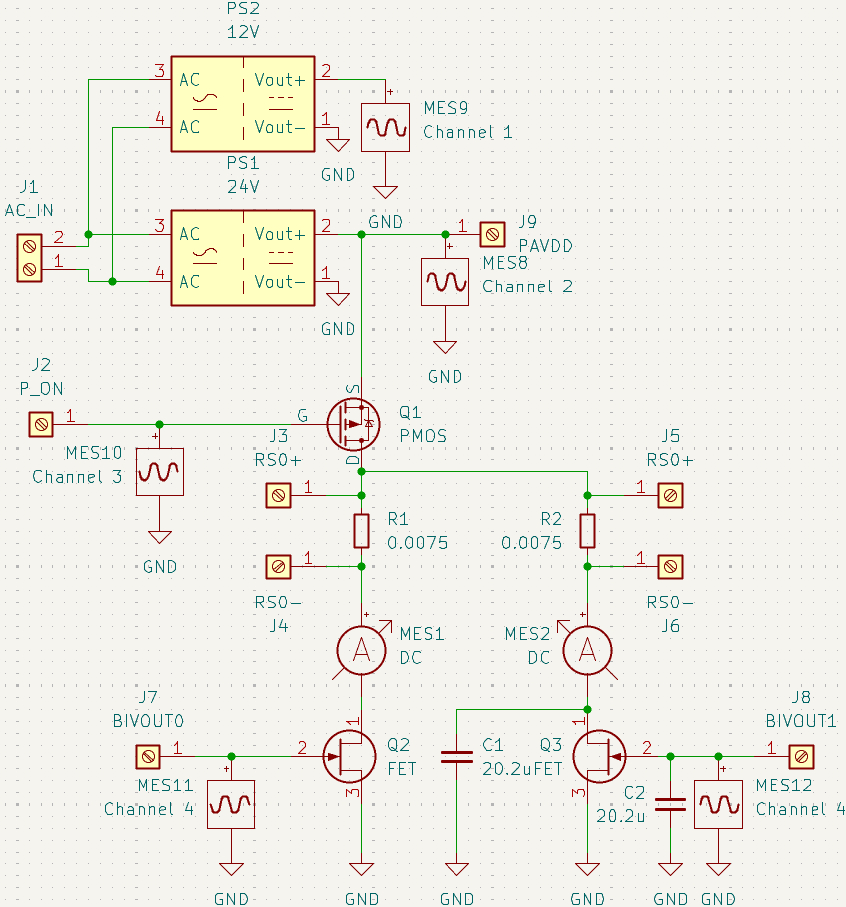
\includegraphics[width=0.8\textwidth]{pictures/test_diagram.png}\hspace{1cm}
    \caption{Darba punkta iestatīšanas/atiestatīšanas testa diagramma}
\end{figure}
Visās oscilogrammās 1. kanāls ir 12 V līnija, 2. kanāls ir 24 V līnija, 3. kanāls ir ieslēgšanas/izslēgšanas vadības signāls un 4. kanāls ir RF jaudas pastiprinātāja aizvara spriegums.
\begin{figure}[H]
	\centering
    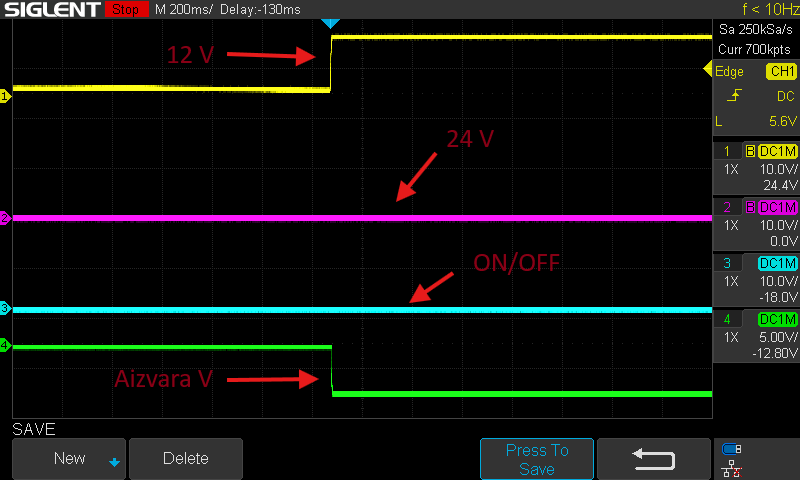
\includegraphics[width=0.9\textwidth]{pictures/device_startup.png}\hspace{1cm}
    \caption{Sistēmas ieslēgšana}
\end{figure}
 3.2. att. ieslēdzoties sistēmai, tiek ieslēgts 12 V barošanas avots, kas nodrošina jaudu visiem 9 V un 5 V patērētājiem, tālāk jaudas pastiprinātāja aizvara spriegums tiek iestatīts uz -5 V, lai to aizvērtu. 24 V barošanas avots netiek ieslēgts, jo to dara  mikrokontrolleris ar manuālu vai tīkla komandu, tāpēc arī nevar novērot 24 V vadības spriegumu ieslēgšanas/izslēgšanas slēdzim.
\begin{figure}[H]
	\centering
    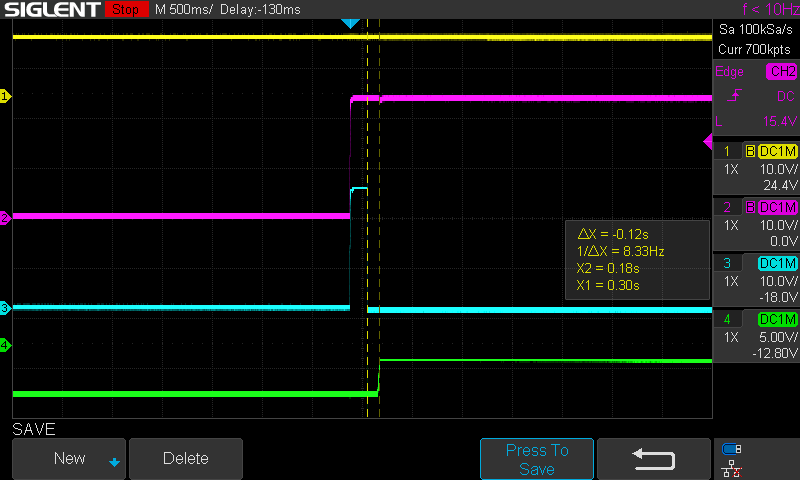
\includegraphics[width=0.9\textwidth]{pictures/load_nocap.png}\hspace{1cm}
    \caption{Sistēmas ieslēgšanās oscilogramma ar testa lauktranzistoru}
\end{figure}
\begin{figure}[H]
	\centering
    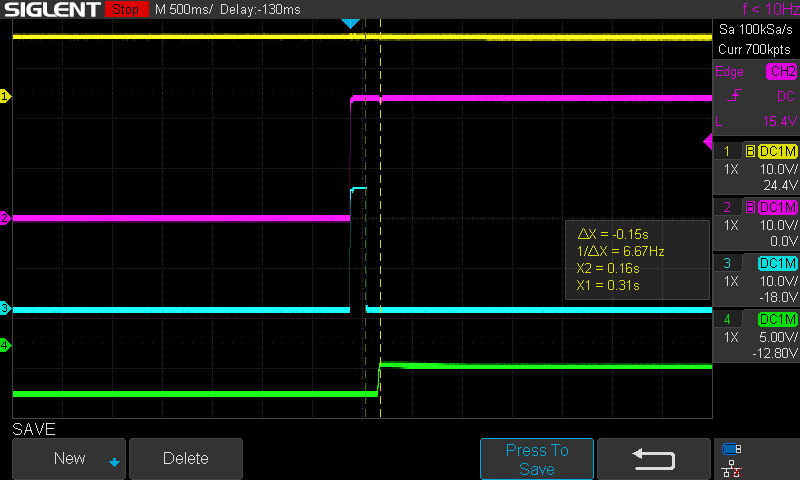
\includegraphics[width=0.9\textwidth]{pictures/capacitive_load.png}\hspace{1cm}
    \caption{Sistēmas ieslēgšanās oscilogramma ar testa lauktranzistoru un filtra kondensatoru}
\end{figure}
3.3. un 3.4. attēlā var redzēt darba punkta iestatīšanu, kur 3.4 attēlā tiek simulēts pats RF pastiprinātājs, pieliekot klāt kondensatorus filtrs. Kad tiek saņemta starta komanda mikrokontrollerī, tad tiek ieslēgts 24 V barošanas avots, kur momentā tiek nodrošināts aizvara spriegums ieslēgšanas/izslēgšanas p-kanāla lauktranzistoram, lai tas būtu aizvērtā stāvoklī. Tad pēc pāris milisekundēm tiek atvērts lauktranzistors un pēc datu lapas nodrošināta vismaz 100 milisekunžu aizture pēc p-kanāla lauktranzistora aktivizēšanas, lai nostabilizētos pārējie procesi.
\begin{figure}[H]
	\centering
    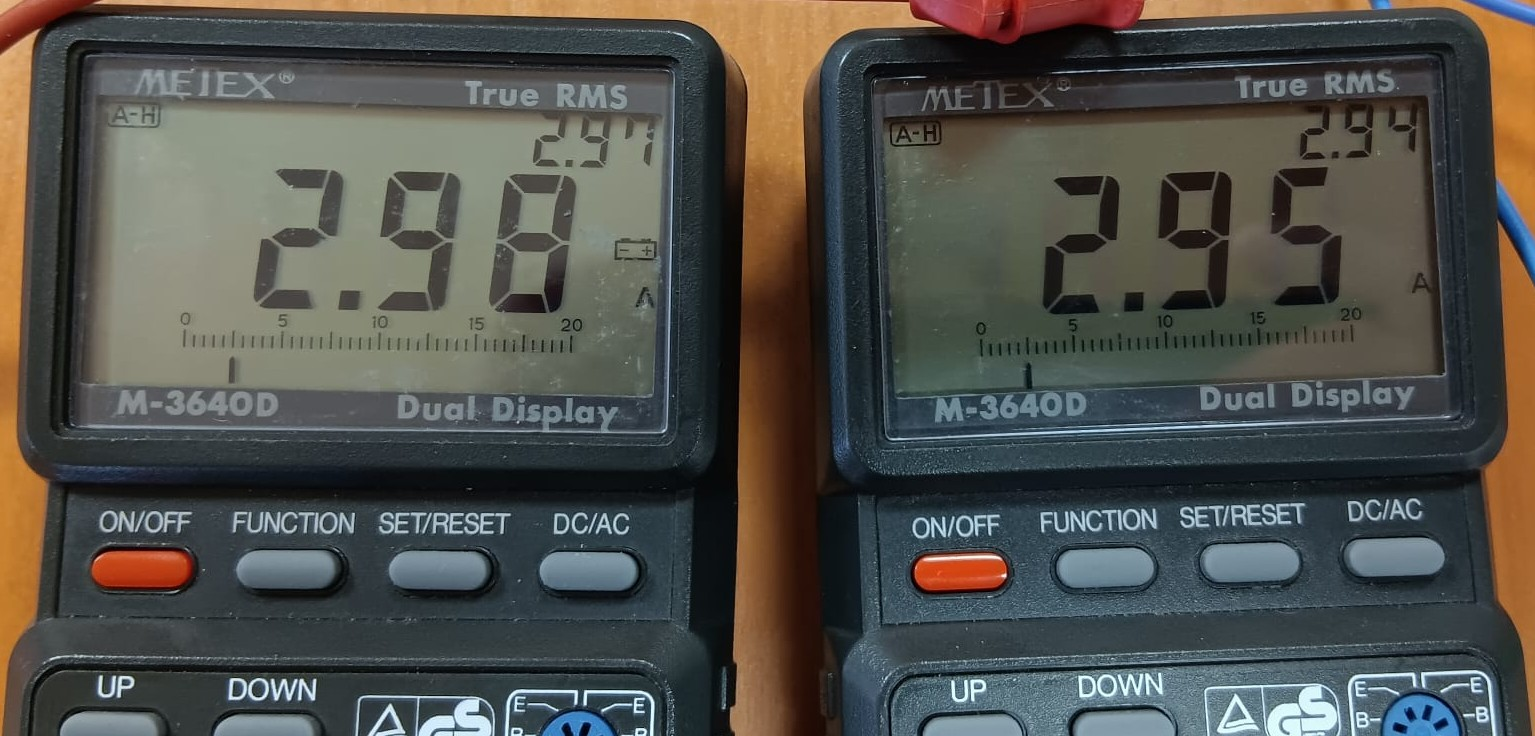
\includegraphics[width=0.9\textwidth]{pictures/load1load2_f.jpg}\hspace{1cm}
    \caption{Noteces strāvas kreisajam un labajam plecam RF jaudas pastiprinātājam}
\end{figure}
3.5. attēlā var redzēt noteces strāvas abiem RF jaudas pastiprinātāja pleciem. Kreisajā pusē 2.98 A tiek nodrošināti testa tranzistoram bez kapacitatīvas slodzes un labajā pusē 2.95 A ar kapacitatīvu slodzi, kas simulē RF jaudas pastiprinātāju.
\begin{figure}[H]
	\centering
    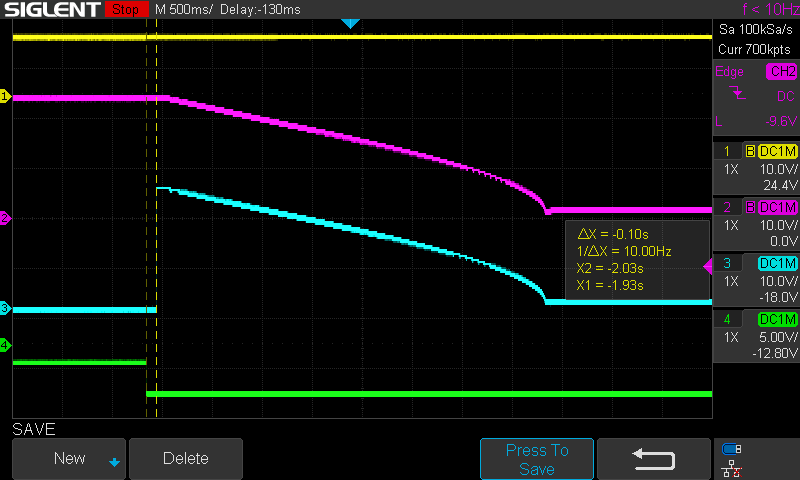
\includegraphics[width=0.9\textwidth]{pictures/load_off_nocap.png}\hspace{1cm}
    \caption{Sistēmas izslēgšana oscilogramma ar testa lauktanzistoru}
\end{figure}
\begin{figure}[H]
	\centering
    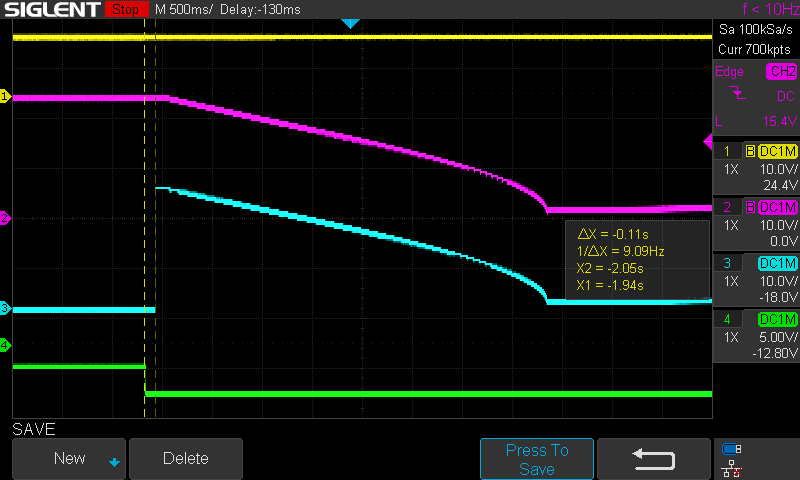
\includegraphics[width=0.9\textwidth]{pictures/cap_load_off.png}\hspace{1cm}
    \caption{Sistēmas ieslēgšanās oscilogramma ar testa lauktanzistoru un filtra kondensatoru}
\end{figure}
3.6. un 3.7. att. var redzēt sistēmas izslēgšanās procesu. Kad tiek saņemta komanda mikrokontrollierī par sistēmas atslēgšanu, tad RF jaudas pastiprinātājam tiek aizvērts, un pēc 100 milisekundēm aizvērts ieslēgšanas / izslēgšanas slēdzis un izslēgts 24 V industriālais barošanas avots.
\begin{figure}[H]
	\centering
    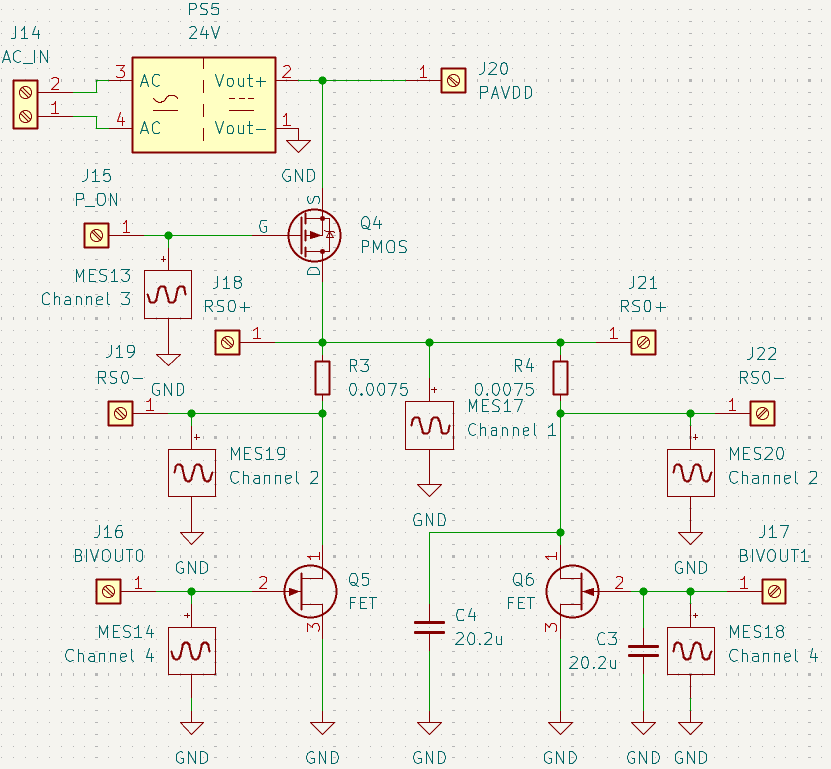
\includegraphics[width=0.8\textwidth]{pictures/test_diagram4.png}\hspace{1cm}
    \caption{Darba punkta iestatīšanas/atiestatīšanas testa diagramma ar differenciālo pāri}
\end{figure}
3.8. att. 1. un 2. kanāls veido diferenciālo pāri, kur tiek mērīts šunta rezistora sprieguma kritums, 3. kanāls mēra vadības signālu ieslēgšanas/izslēgšanas slēdzim un 4. kanāls aizvara spriegumu jaudas pastiprinātājam.
\begin{figure}[H]
	\centering
    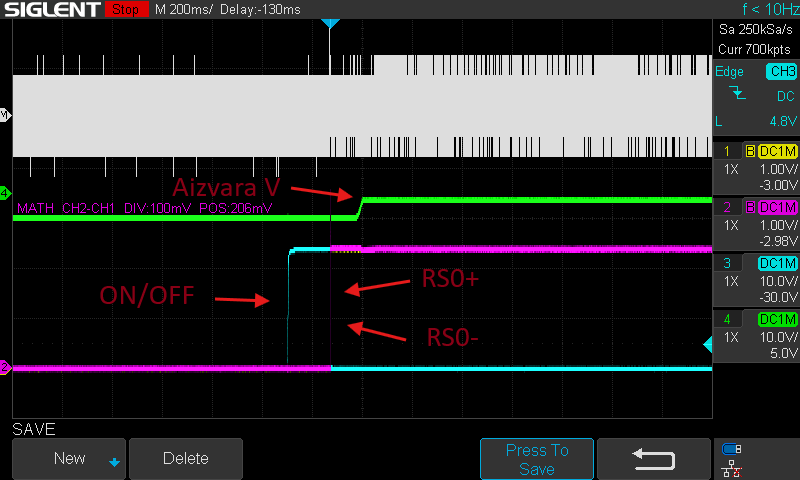
\includegraphics[width=0.9\textwidth]{pictures/current.png}\hspace{1cm}
    \caption{Sprieguma krituma noteikšana uz šunta rezistora}
\end{figure}
 Osciloskopam mazākajā mērīšanas diapazonā ir mazāki kanāla trokšņi, tāpēc osciloskopa tausti tika iestatīti uz 10x un osciloskopā nokonfigurēts uz 1x, lai varētu mērīt lielāku signālu ar mazāku sprieguma diapazonu, bet, neskatoties uz to, 1V mērīšanas diapozonam ir 100 mV pk-pk troksnis, tādēļ nebija iespējams izmērīt 22 mV sprieguma kritumu uz šunta rezistora, bet, kad beidzas pārejas process, tad var redzēt, ka troksnis sāk svārstīties ap citu vērtību, bet tas nedod noteiktu vērtību.
\section{Elektrobarošanas plates testi}
Testā tika novērtēts iekārtu jaudas patēriņš un elektrobarošanas risinājuma novērtējums.
\begin{figure}[H]
	\centering
    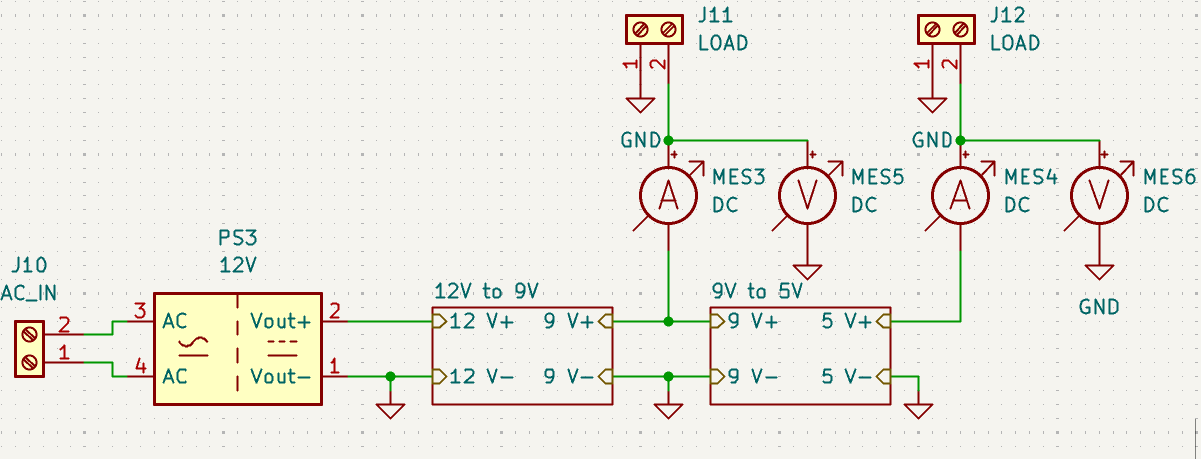
\includegraphics[width=0.9\textwidth]{pictures/test_diagram2.png}\hspace{1cm}
    \caption{9 un 5 V barošanas testa diagramma}
\end{figure}
3.9. att. redzams testa iekārtu slēgums elektriski principiālajā ķēdē un slodzes pieslēguma vieta.
\begin{table}[H]
\captionsetup{singlelinecheck=off, justification=raggedleft}
\caption{9 V elektrobarošanas}
\centering
\begin{tabular}{|c|c|c|c|c|c|}
\hline
\multicolumn{2}{|c|}{\makecell{Ieejas parametri}} 
& \multicolumn{2}{c|}{\makecell{Izejas parametri}} 
& \multirow{2}{*}{\makecell{Slodze, \si{\ohm}}} 
& \multirow{2}{*}{\makecell{Eff, \%}} \\
\cline{0-3}
\makecell{Spriegums, \si{\volt}} 
& \makecell{Strāva, \si{\ampere}}
& \makecell{Spriegums, \si{\volt}}
& \makecell{Strāva, \si{\ampere}}
&  &\\ 
\hline
12.04\pm0.12 & 0.02\pm0.01 & 8.95\pm0.01 & 0.01\pm0.00 & 14280.00\pm0.00 & 37.16 \\ 
\hline
12.06\pm0.12 & 0.12\pm0.01 & 8.96\pm0.01 & 0.10\pm0.00 & 90.14\pm0.00 & 61.91 \\ 
\hline
12.02\pm0.12 & 0.22\pm0.01 & 8.96\pm0.01 & 0.20\pm0.00 & 44.84\pm0.00 & 67.76 \\ 
\hline
12.03\pm0.12 & 0.32\pm0.02 & 8.98\pm0.01 & 0.30\pm0.00 & 29.90\pm0.00 & 69.98 \\ 
\hline
12.03\pm0.12 & 0.42\pm0.02 & 8.98\pm0.01 & 0.40\pm0.00 & 22.44\pm0.00 & 70.09 \\ 
\hline
12.00\pm0.12 & 0.53\pm0.02 & 8.99\pm0.01 & 0.50\pm0.00 & 17.96\pm0.00 & 70.68 \\ 
\hline
11.99\pm0.12 & 0.63\pm0.02 & 8.99\pm0.01 & 0.60\pm0.00 & 14.98\pm0.00 & 71.40 \\ 
\hline
11.98\pm0.12 & 0.73\pm0.02 & 9.00\pm0.01 & 0.70\pm0.00 & 12.85\pm0.00 & 72.04 \\ 
\hline
11.98\pm0.12 & 0.83\pm0.02 & 9.00\pm0.01 & 0.80\pm0.00 & 11.25\pm0.00 & 72.41 \\ 
\hline
11.97\pm0.12 & 0.93\pm0.03 & 9.00\pm0.01 & 0.90\pm0.00 & 10.01\pm0.00 & 72.76 \\ 
\hline
11.96\pm0.12 & 1.03\pm0.03 & 9.00\pm0.01 & 1.00\pm0.00 & 8.99\pm0.00 & 73.06 \\ 
\hline
\end{tabular}
\end{table}

Izveidotais 9 V pārveidotāja risinājums spēj nodrošināt nepieciešamo jaudu slodzei.

\begin{table}[H]
\centering
\captionsetup{singlelinecheck=off, justification=raggedleft}
\caption{5 V elektrobarošanas}
\begin{tabular}{|c|c|c|c|c|c|}
\hline
\multicolumn{2}{|c|}{\makecell{Ieejas parametri}} 
& \multicolumn{2}{c|}{\makecell{Izejas parametri}} 
& \multirow{2}{*}{\makecell{Slodze, \si{\ohm}}} 
& \multirow{2}{*}{\makecell{Eff, \%}} \\
\cline{0-3}
\makecell{Spriegums, \si{\volt}} 
& \makecell{Strāva, \si{\ampere}}
& \makecell{Spriegums, \si{\volt}}
& \makecell{Strāva, \si{\ampere}}
&  &\\ 
\hline
8.95\pm0.01 & 0.02\pm0.01 & 5.15\pm0.01 & 0.01\pm0.00 & 13020.00\pm0.00 &  28.61 \\ 
\hline
8.96\pm0.01 & 0.11\pm0.01 & 5.15\pm0.01 & 0.10\pm0.00 & 51.22\pm0.00 & 52.02 \\ 
\hline
8.96\pm0.01 & 0.21\pm0.01 & 5.16\pm0.01 & 0.20\pm0.00 & 25.70\pm0.00 & 54.50 \\ 
\hline
8.98\pm0.01 & 0.31\pm0.02 & 5.16\pm0.01 & 0.30\pm0.00 & 17.19\pm0.00 & 55.37 \\ 
\hline
8.98\pm0.01 & 0.41\pm0.02 & 5.16\pm0.01 & 0.40\pm0.00 & 12.89\pm0.00 & 56.10 \\ 
\hline
8.99\pm0.01 & 0.51\pm0.02 & 5.16\pm0.01 & 0.50\pm0.00 & 10.31\pm0.00 & 56.28 \\ 
\hline
8.99\pm0.01 & 0.61\pm0.02 & 5.16\pm0.01 & 0.60\pm0.00 & 8.59\pm0.00 & 56.42 \\ 
\hline
9.00\pm0.01 & 0.71\pm0.02 & 5.15\pm0.01 & 0.70\pm0.00 & 7.35\pm0.00 & 54.87 \\ 
\hline
9.00\pm0.01 & 0.81\pm0.02 & 5.14\pm0.01 & 0.80\pm0.00 & 6.43\pm0.00 & 56.52 \\ 
\hline
9.00\pm0.01 & 0.91\pm0.03 & 5.15\pm0.01 & 0.90\pm0.00 & 5.72\pm0.00 & 56.60 \\ 
\hline
9.00\pm0.01 & 1.01\pm0.03 & 5.15\pm0.01 & 1.00\pm0.00 & 5.14\pm0.00 & 56.66 \\ 
\hline
\end{tabular}
\end{table}

Izveidotais 5 V pārveidotāja risinājums spēj nodrošināt nepieciešamo jaudu slodzei. Slēdzot to kaskādes slēgumā pēc 9 V elektrobarošanas avota, tiek paaugstināta lineārā sprieguma efektivitāte, jo ir mazāk jaudas jāizkliedē uz sevis.

\begin{figure}[H]
\centering
\begin{tikzpicture}
\begin{axis}[
    title={Sprieguma atkarība no slodzes},
    xlabel={Strāva (\si{\ampere})},
    ylabel={Spriegums (\si{\volt})},
    xmin=0, xmax=1,
    ymin=0, ymax=10,
    grid=both,
    grid style={line width=0.1pt, draw=gray!50},
    width=0.8\textwidth,
    axis lines=left,
    legend pos=north west,
]

% Line 1: 9V (Red)
\addplot[
    color=red,
    mark=*,
    line width=1pt,
]
coordinates {
    (0, 8.987)
    (0.1, 8.985)
    (0.2, 8.983)
    (0.3, 8.985)
    (0.4, 8.990)
    (0.5, 8.991)
    (0.6, 8.985)
    (0.7, 8.982)
    (0.8, 8.981)
    (0.9, 8.980)
    (1, 8.979)
};
\addlegendentry{9V}

% Line 2: 5V (Blue)
\addplot[
    color=blue,
    mark=square*,
    dashed,
    line width=1pt,
]
coordinates {
    (0, 5.168)
    (0.1, 5.165)
    (0.2, 5.163)
    (0.3, 5.161)
    (0.4, 5.160)
    (0.5, 5.160)
    (0.6, 5.159)
    (0.7, 5.158)
    (0.8, 5.157)
    (0.9, 5.155)
    (1, 5.153)
};
\addlegendentry{5V}

\end{axis}
\end{tikzpicture}
\caption{Strāvas-sprieguma raksturlīkne 9V un elektrobarošanas līnijām}
\end{figure}
Grafiski atveidoti iegūtie rezultāti. Maksimālais strāvas patēriņš 9 V līnijai ir 310 mA un 5 V līnijai 110 mA.
\section{True RMS jaudas detektora un RF kabeļu tests}
S-parametru noteikšanai tiek veikti no 6.5 līdz 8.5 GHz diapozonā. Tiek veikts koaksiālo kabeļu RFC1 un RFC2 S-parametru (skat. att. 2.1.), kas savieno atzarotāja $P_{fwd}$ un $P_{ref}$ ar jaudas detektoru un jaudas detektora novērtējums. Tad jaudas detektora izejas sprieguma atkarība no ieejas signāla jaudas pie 7.2 GHz.
\begin{figure}[H]
	\centering
    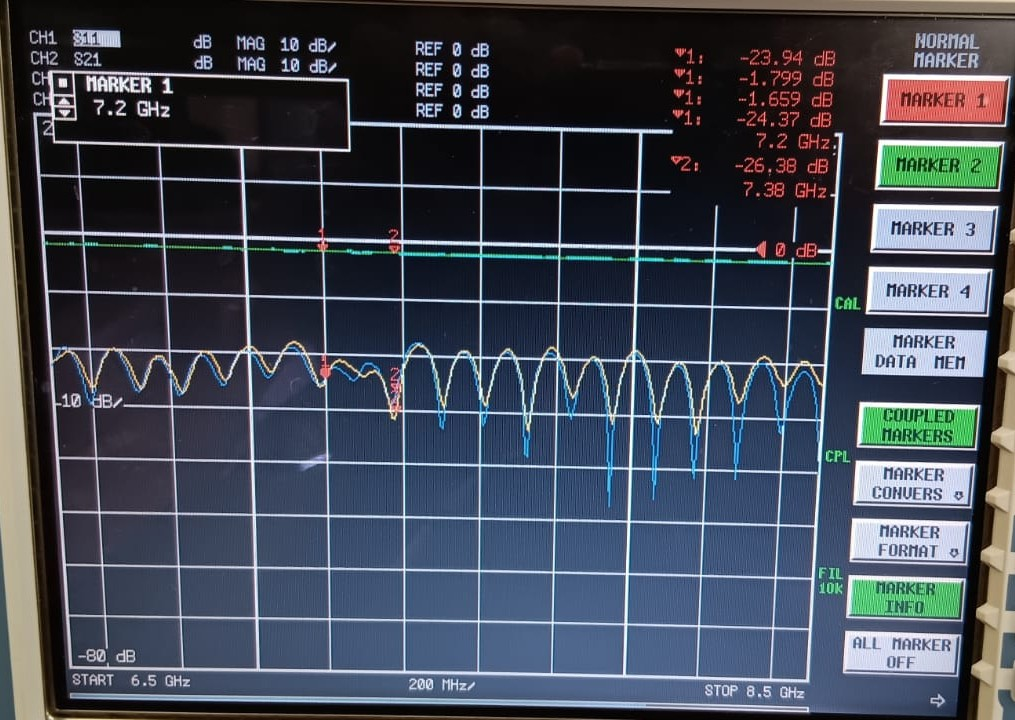
\includegraphics[width=0.7\textwidth]{pictures/cable_coax_fwd.jpg}\hspace{1cm}
    \caption{Izstarotās jaudas koaksiālais kabeļa S-parametri}
\end{figure}
Lielākā daļa no ienākošās jaudas koaksiālajā kabelī netiek atstarota ($S_{11}$ un $S_{22}$) atpakaļ -24 dB, kas ir aptuveni 0.4\% no jaudas, bet, neskatoties uz to, pašā vadā ir -1.8 dB zudums ($S_{21}$ un $S_{12}$), kas ir aptuveni 33\% no ienākošās jaudas.
\begin{figure}[H]
	\centering
    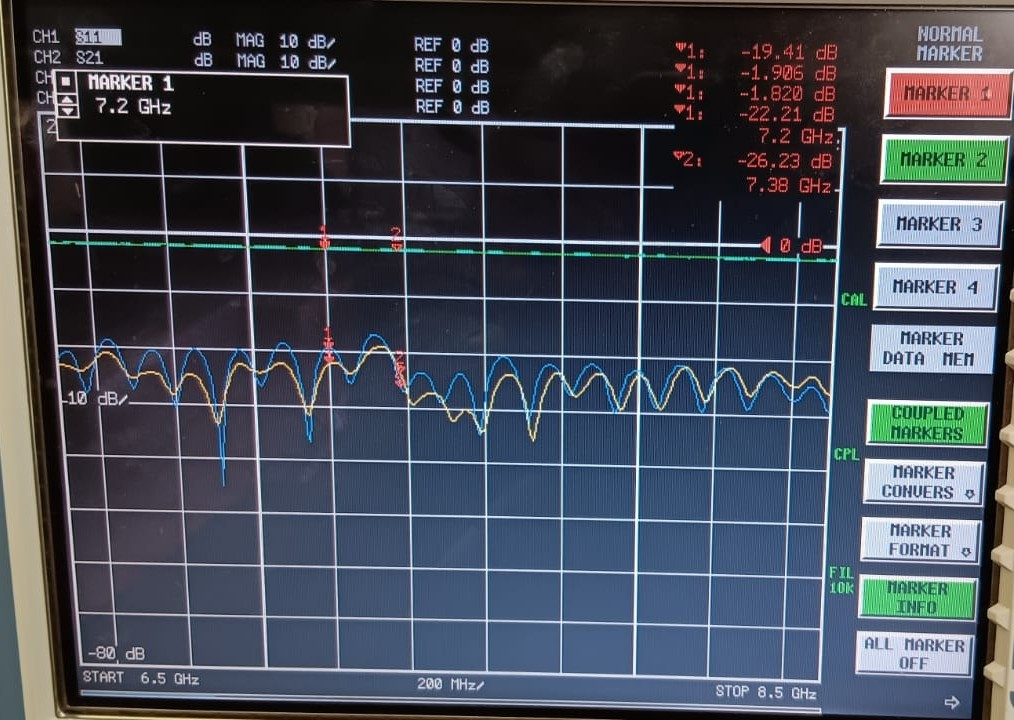
\includegraphics[width=0.7\textwidth]{pictures/cable_coax_ref.jpg}\hspace{1cm}
    \caption{Atstarotās jaudas koaksiālais kabelā S-parametri}
\end{figure}
Lielākā daļa no ienākošās jaudas koaksiālajā kabelī netiek atstarota ($S_{11}$ un $S_{22}$) atpakaļ -20 dB, kas ir aptuveni 1\% no jaudas, bet, neskatoties uz to, pašā kabelī ir -1.9 dB zudums ($S_{21}$ un $S_{12}$), kas ir aptuveni 36\% no ienākošās jaudas.
\begin{figure}[H]
	\centering
    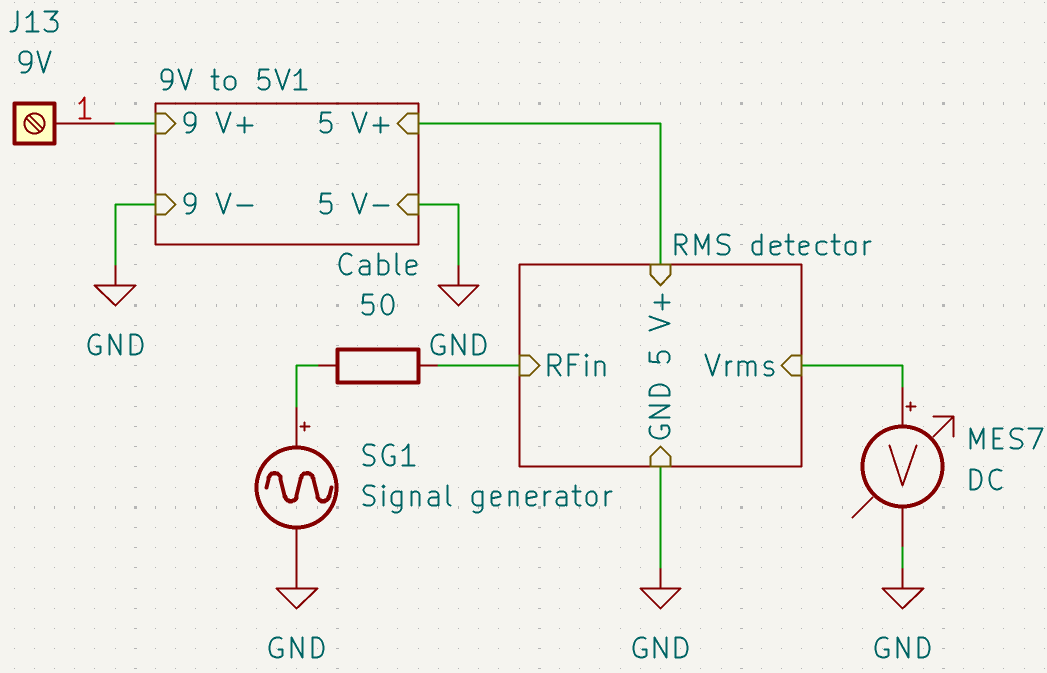
\includegraphics[width=0.7\textwidth]{pictures/tests_diagram3.png}\hspace{1cm}
    \caption{Jaudas detektora testu diagramma}
\end{figure}
3.14. att. redzams testa iekārtu slēgums elektriski principiālajā shēmā.
\begin{figure}[H]
	\centering
    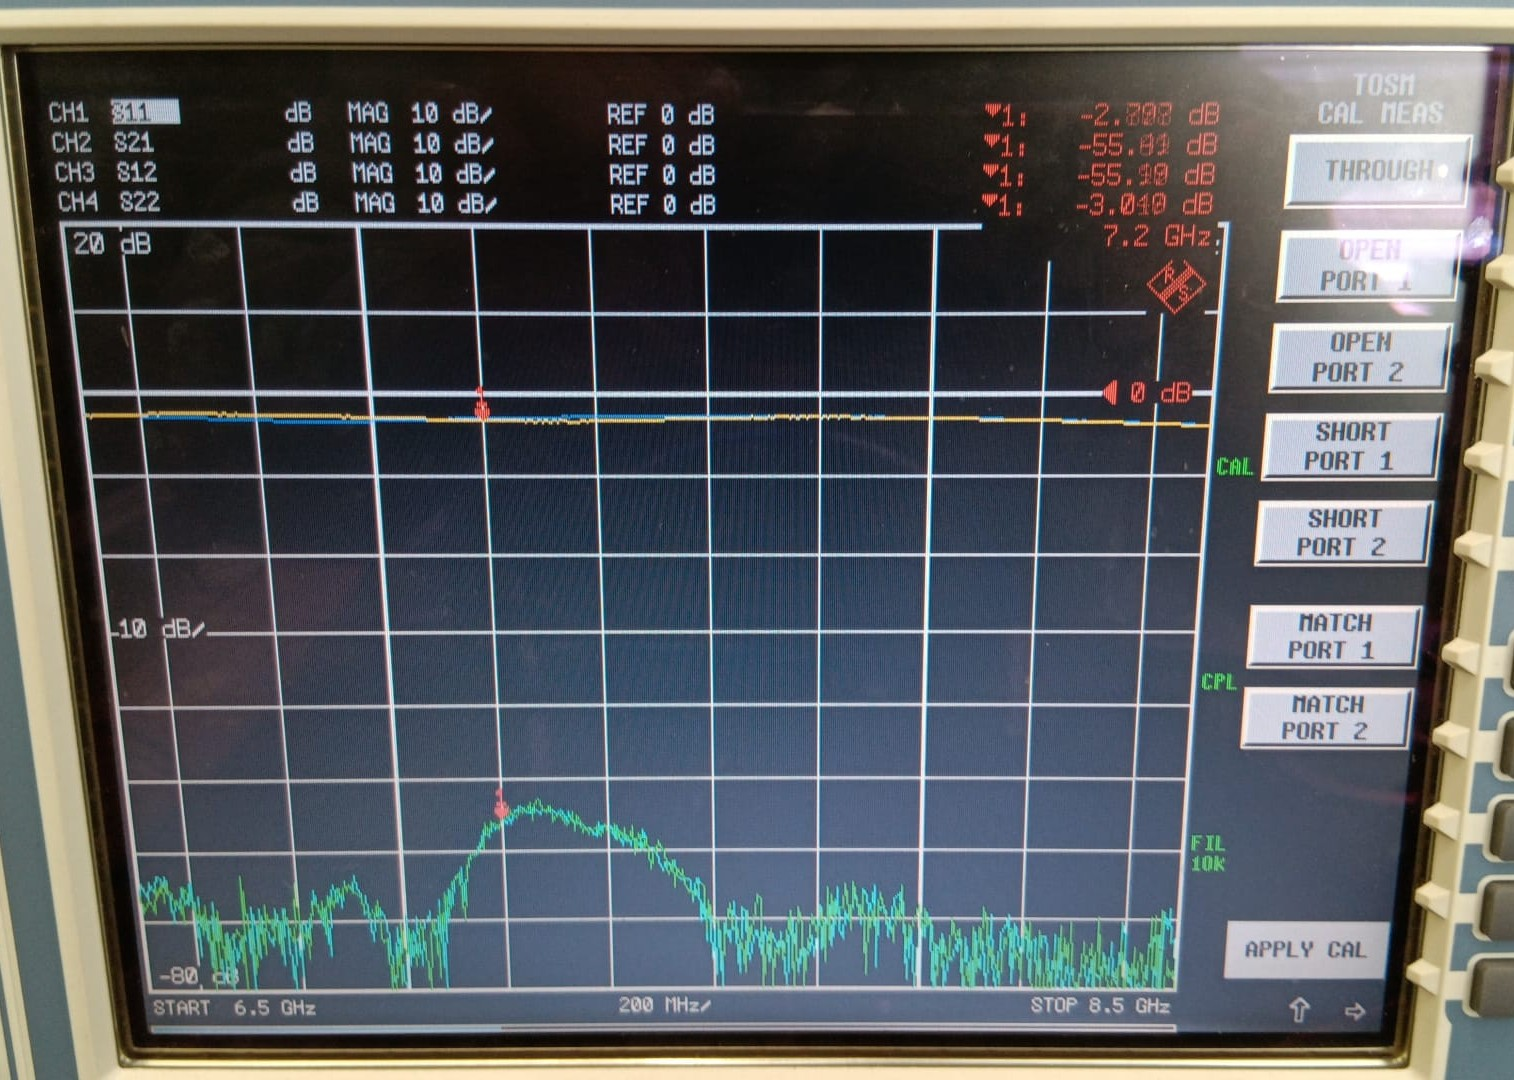
\includegraphics[width=0.7\textwidth]{pictures/vna_measurement_powerdet.jpeg}\hspace{1cm}
    \caption{S-parametri jaudas detektoram}
\end{figure}
Izstarotā un atstarotā jaudas kanāli atstaro aptuveni pusi no ienākošā signāla jaudas. Savstarpējā portu izolācija ir laba, kas tiek panākta ar metalizētiem urbumiem.
\begin{figure}[H]
\centering
\begin{tikzpicture}
\begin{axis}[
    title={Sprieguma līmenis atkarībā no ieejas jaudas},
    xlabel={Jauda (dBm) },
    ylabel={Spriegums (\si{\volt})},
    xmin=-60, xmax=20,
    ymin=0, ymax=2,
    grid=both,
    grid style={line width=0.1pt, draw=gray!50},
    width=0.8\textwidth,
    axis lines=left,
    legend pos=north west,
]

% Line 1: FWD power (Red)
\addplot[
    color=red,
    mark=*,
    line width=1pt,
]
coordinates {
    (-50, 0.104)
    (-49, 0.215)
    (-48, 0.250)
    (-47, 0.279)
    (-46, 0.303)
    (-45, 0.328)
    (-44, 0.350)
    (-43, 0.375)
    (-42, 0.397)
    (-39, 0.466)
    (-36, 0.559)
    (-33, 0.641)
    (-30, 0.754)
    (-27, 0.859)
    (-24, 0.952)
    (-21, 1.048)
    (-18, 1.143)
    (-15, 1.224)
    (-12, 1.347)
    (-9, 1.463)
    (-6, 1.583)
    (-3, 1.672)
    (0, 1.757)
    (3, 1.818)
    (6, 1.863)
    (9, 1.879)
    (10, 1.867)
};
\addlegendentry{Izstarotā jauda}

% Line 2: REF power (Blue)
\addplot[
    color=blue,
    mark=square*,
    dashed,
    line width=1pt,
]
coordinates {
    (-55, 0.355)
    (-54, 0.358)
    (-53, 0.366)
    (-52, 0.368)
    (-51, 0.373)
    (-50, 0.377)
    (-49, 0.382)
    (-48, 0.388)
    (-47, 0.394)
    (-46, 0.403)
    (-45, 0.412)
    (-44, 0.420)
    (-43, 0.431)
    (-42, 0.442)
    (-41, 0.454)
    (-40, 0.466)
    (-39, 0.484)
    (-36, 0.554)
    (-33, 0.636)
    (-30, 0.733)
    (-27, 0.822)
    (-24, 0.914)
    (-21, 1.000)
    (-18, 1.098)
    (-15, 1.175)
    (-12, 1.284)
    (-9, 1.394)
    (-6, 1.503)
    (-3, 1.613)
    (0, 1.686)
    (3, 1.768)
    (6, 1.831)
    (9, 1.920)
    (10, 1.855)
};
\addlegendentry{Atstarotā jauda}

\end{axis}
\end{tikzpicture}
\caption{Izejas sprieguma ietekme uz ieejas jaudu}
\end{figure}
Iegūstot izejas sprieguma līmeņu atkarības no ieejas jaudas, tika ņemti vērā signāla ģeneratora un vada zudumi. Līkne, kas tika iegūta abos kanālos, ir ļoti līdzīga ražotāja dotajai specifikācijai. Jutības diapazons ir no -50 līdz 9 dBm, kur 0 dBm atbilst 100 W, tad mēs varam izmērīt no 1 mW līdz 794,3 W.
\section{Tīkla testi}
Šajā testā tiek pārbaudīta vadības sistēma no operatora datora līdz mikrokontrolieram ar skripta palīdzību, kas rakstīts Python priekš Windows OS. Tests tika veikts izolētā tīklā, kur atradās tikai divas ierīces: operātora dators un mikrokontrolieris ar visu X-joslas sistēmu.
\begin{figure}[H]
	\centering
    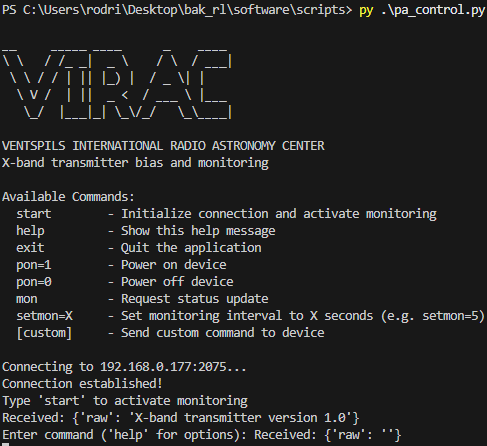
\includegraphics[width=0.9\textwidth]{pictures/script_start.png}\hspace{1cm}
    \caption{Klienta konfigurēšana lokālajā tīklā}
\end{figure}
Tests sākās ar skripta uzsākšanu. Terminālī redzams logo, palīgrinda un to, ka veiksmīgi ir pieslēdzies pie TCP servera, kurš uzreiz pēc pieslēgšanās atsūta savu nosaukumu un versiju. Tad lietotājam tiek sniegta informācija par komandu, kura uzsāk monitorēšanu un darba punkta iestatīšanu. Pēc tā tiek aicināts ievadīt komandu.
\begin{figure}[H]
	\centering
    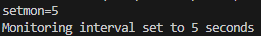
\includegraphics[width=0.9\textwidth]{pictures/script_monchange.png}\hspace{1cm}
    \caption{Monitorēšanas cikla aizkaves maiņa}
\end{figure}
Redzams monitorēšanas intervāla iestatīšanu no noklusētās vērtības 30 sec uz 5 sekundēm.
\begin{figure}[H]
	\centering
    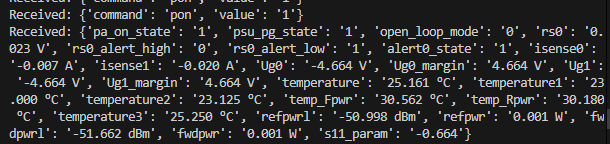
\includegraphics[width=0.9\textwidth]{pictures/script_system_start .png}\hspace{1cm}
    \caption{Darba punkta iestatīšana un telemetrijas virkne}
\end{figure}
Tad tika uzsākta sistēmas darbība ar komandu "start", kur var redzēt, ka tika nosūtīta komanda pon=1 un saņemta atbilde no mikrokontroliera pon=1, kas liecina par to, ka komanda tika saņemta un veiksmīgi apstrādāta. Pēc kā seko monitorēšanas telemetrijas ik pēc 5 sekundēm.
\begin{figure}[H]
	\centering
    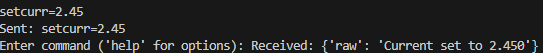
\includegraphics[width=0.9\textwidth]{pictures/script_setcurr.png}\hspace{1cm}
    \caption{Darba punkta noteces strāvas iestatīšana}
\end{figure}
\begin{figure}[H]
Tad tiek iestatīts cita darba punkta strāva no 3 A uz 2.45 A, kur mikrokontrolieris arī deva atbildi, ka tā tika veiksmīgi uzstādīta.
	\centering
    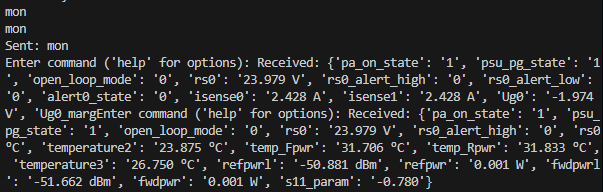
\includegraphics[width=0.9\textwidth]{pictures/script_setcurr_tel.png}\hspace{1cm}
    \caption{Strāvas maiņas telemetrijas virkne}
\end{figure}
Tad var redzēt, ka telemetrijas virknē ir aizvara spriegums cits un noteces strāva 2.426 A.
\begin{figure}[H]
	\centering
    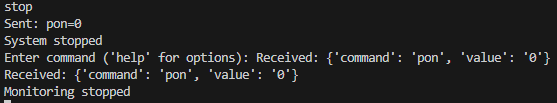
\includegraphics[width=0.9\textwidth]{pictures/script_system_stop.png}\hspace{1cm}
    \caption{Darba punkta atiestatīšana}
\end{figure}
Aktīvu sistēmu var deaktivizēt ar komandas nosūtīšanu "stop", kas uzreiz uz mikrokontrolieri nosūta komandu pon=0 un izbeidz monitorēšanas pavedienu.
\begin{figure}[H]
	\centering
    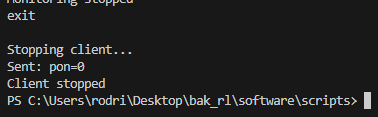
\includegraphics[width=0.9\textwidth]{pictures/script_exit.png}\hspace{1cm}
    \caption{Skripta izslēgšana}
\end{figure}
Ar exit vai ctrl+c var izbeigt skripta darbību, kur tiek aizsūtīta komanda pon=0, lai izslēgtu sistēmu, ja tā bija aktīva, un atvienojas no servera, tad izbeidz visu aktīvo pavedienu darbību.


\chapter{Secinājumi un priekšlikumi}

\bibliography{refs}
%\input{pielikumi.tex}
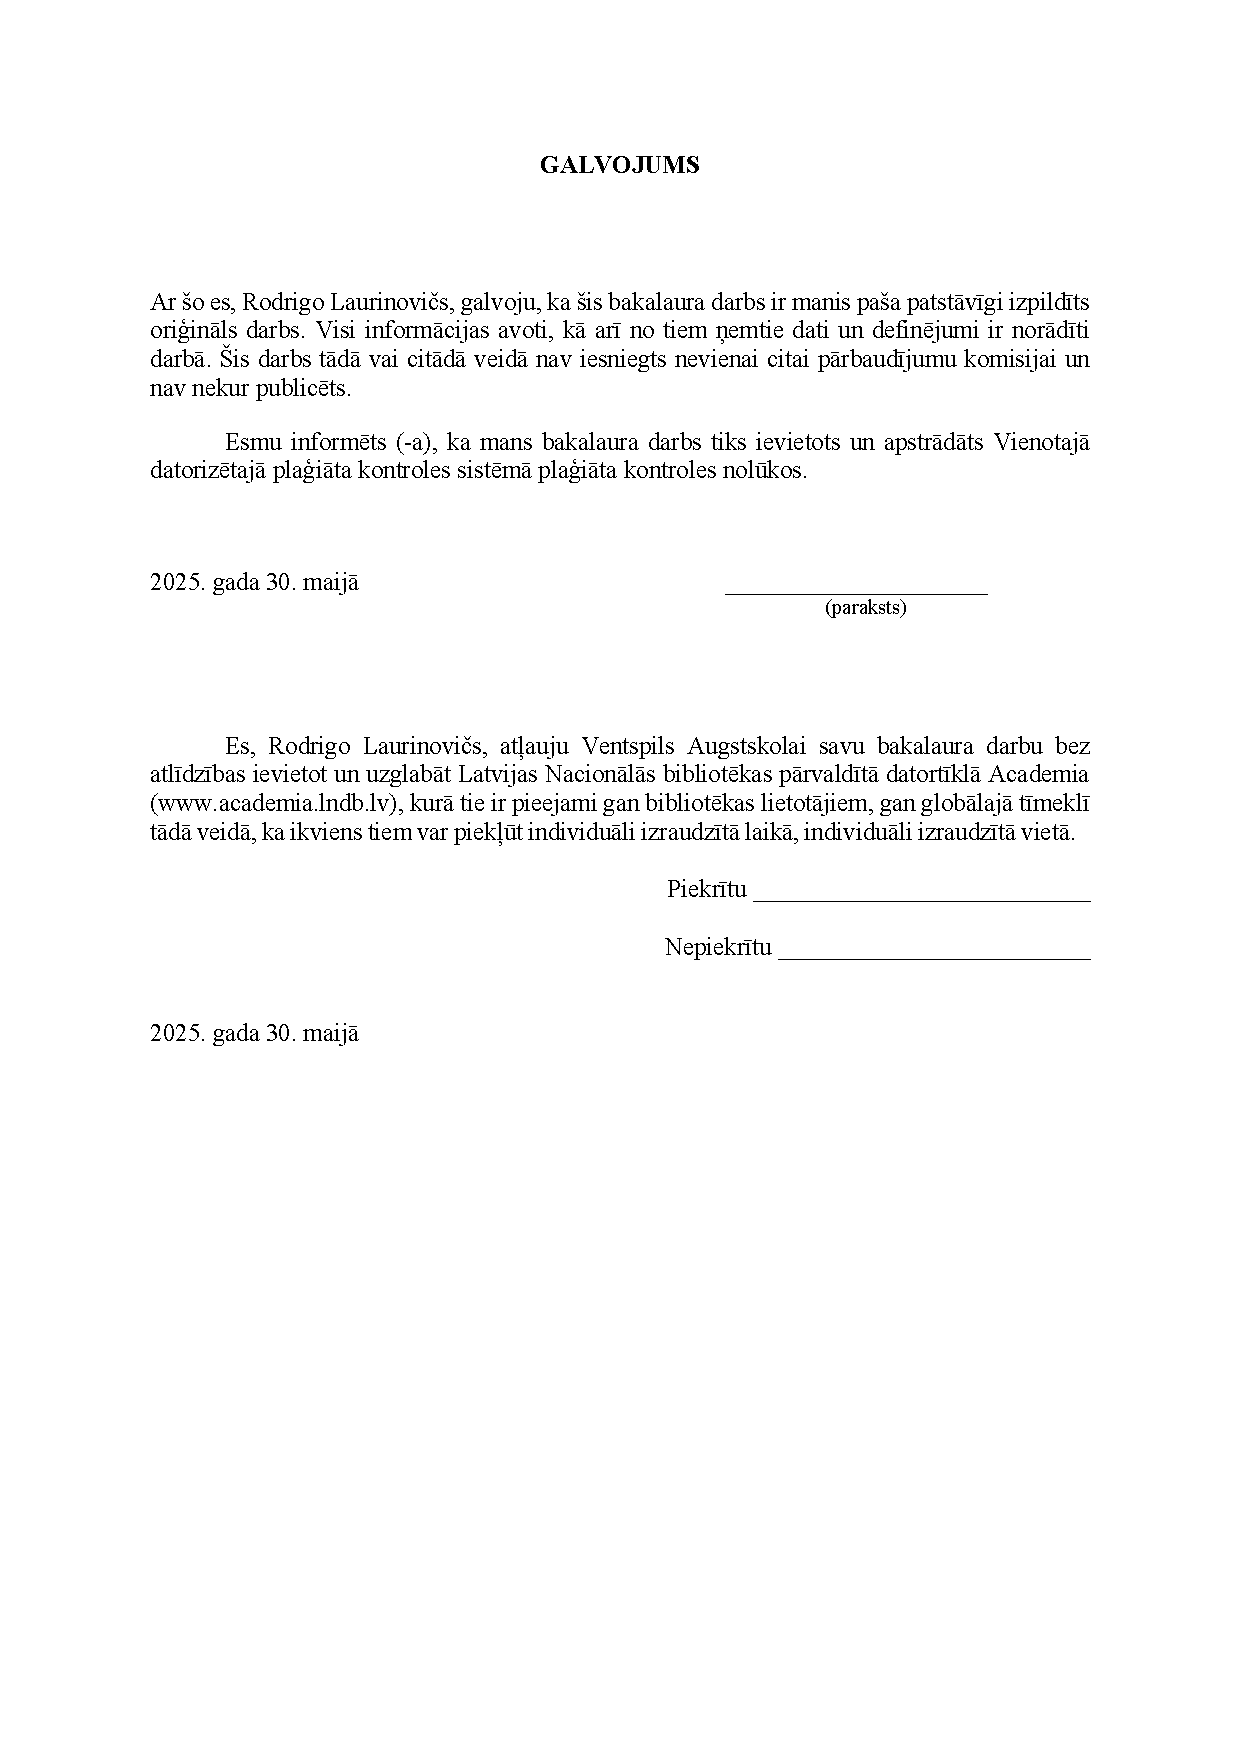
\includepdf[pages=-]{Galvojums.pdf}

\end{document}
